%/**********************************************************************/
%		第4章:マルチポートCAMベース並列テーブルルックアップ符号化アーキテクチャ
%/**********************************************************************/
\chapter{マルチポートCAMベース並列テーブルルックアップ符号化処理}
\label{lbl_chptr4}

本章では,マルチメディアデータを高速に処理するための,
ボトルネックとなっていたテーブルルックアップ処理を,
並列度の向上によって解決する手法を提案する.
並列にテーブルルックアップ処理を実現するアーキテクチャとして,
フレキシブルマルチポートCAM (FMCAM: Flexible Multi-Ported Content Addressable Memory)を提案する
\cite{kummmc01, kumkaij, kumpro, kumfle04j, kummva05, kumfmc06, kumsfi06}.
FMCAMは,従来効率よい処理が困難であった並列一致検索処理を実現可能にした,新しい機能メモリである.

本章の構成は,\ref{lbl_cp4_intro}節において,テーブルルックアップ処理を並列化することの
意義について述べる.
\ref{lbl_cp4_fmcam}節では,FMCAMのアーキテクチャについて詳述し,FPGAへの実装を通して性能評価を行う.
次に,\ref{lbl_cp4_adpt_fmcam}節において,汎用向けアーキテクチャであったFMCAMをテーブルルックアップ処理向けに特化した
改良について説明する.
\ref{lbl_cp4_adpt_fmcam_arch}節では,改良されたFMCAMのアーキテクチャを詳述し,
\ref{lbl_cp4_adpt_fmcam_impl}節において,FPGA及びASICへの実装を通して性能評価を行う.
\ref{lbl_cp4_adpt_fmcam_huffma}節では,テーブルルックアップ処理の1つであるハフマン符号化に着目し,
FMCAMの処理能力を検証する.
また,\ref{lbl_cp4_adpt_fmcam_ophu}節では,提案アーキテクチャと,\ref{lbl_chptr3}章で述べた
リアルタイム符号化テーブル最適化アーキテクチャの融合について検討する.
最後に,\ref{lbl_cp4_matome}節にて本章のまとめを述べる.

%/**********************************************************************/
%		イントロの章
%/**********************************************************************/
\section{はじめに}
\label{lbl_cp4_intro}
マルチメディアデータを高速に処理するためには
テーブルルックアップ処理を高速に行うことが必須である.
一般に,高速化の方法で代表的なものは並列化が
考えられるが,テーブルルックアップ処理を並列化する場合,
符号化のためのテーブルを複数用意する必要がある.
しかし,この方法では面積及び消費電力が大きくなり,
テーブルデータ間のコヒーレンシや同期等の問題も無視することはできない.
そのため,これまでのマルチメディアデータ処理LSIは,
主にパイプライン処理によって高速化を図っていた
\cite{seuema99, cmjamp, shaecs88, musdcw98}.
しかしながら,図 \ref{huf_arch}で示したように,テーブルルックアップ
処理は別モジュールで行われることが多く,データ転送の際に
内部バスの混雑を生じさせ,消費電力も増大する結果となる.
加えて近年の汎用プロセッサやメディアプロセッサは処理能力向上のために,
演算器を並列に複数備えるアーキテクチャや
コアを複数備えるマルチコア化が進んでいる\cite{jorpje, hjfr5505}.
これらのアーキテクチャの発展に,テーブルルックアップ処理を適合させるには,
これまで実現が困難であった並列化の実現が求められる.
そこで,本章では,テーブルルックアップ処理の
高速処理のために,従来のCAMに比較ポートを複数実装させた
マルチポートCAMを新たに開発し,
マルチポートCAMを適用した並列テーブルルックアップ符号化アーキテクチャと,その有効性を示す.
%/**********************************************************************/
%		FMCAMの説明
%		該当論文: ieice_j_fmcam
%/**********************************************************************/
\section{フレキシブルマルチポートCAM}
\label{lbl_cp4_fmcam}
	本章では,CAMの能力向上の一手法として,マルチポート化に着目し,
	新しいCAMアーキテクチャであるフレキシブルマルチポートCAMであるFMCAM (Flexible Multi-ported Content Addressable Memory)を
	提案する.
	性能評価のためにFMCAMをFPGAに実装することにより,既存のCAMとの比較を通して,処理能力の向上及びハードウェア量の削減効果を示す.

\subsection{CAMのマルチポート化}
\label{lbl_cp4_cam_multi}

\subsubsection{マルチポート化への背景}
\label{lbl_cp4_cam_haikei}
	CAMは機能メモリの一種であり,
	主として一致検索処理を実行する回路である.
	一般にCAMは,その一致検索能力が高速であることが知られているが,
	実際には処理速度と比較器の数の関係,及びコストの問題があり,これらが普及の妨げになっている.
	ここで,	CAMの能力を向上させる方法として考えられるのは,
	最大動作周波数の向上,処理ビット幅の拡大,及びポート数の増加の3点であり,
	特にポート数の増加は,その他の方法と比較して有効であることが示されている \cite{hukban}.
	この観点から既存のCAMをポート数で大別した場合,(1)入力ポート及び出力ポートを1対持ち比較対象データを格納する内部のメモリである
	コンテンツテーブルを1つ持つシングルポートCAM,(2)複数の入力ポートと1つの出力ポートを持ちコンテンツテーブルを
	共有しているマルチインプットCAM \cite{harcol},及び(3)シングルポートのCAMを並列に配置した
	並列CAMの3つがあげられる.
	特に,大規模なアプリケーションほど並列CAMにより処理能力の向上を図っているものが多い 
	\cite{ccocis, hardet, harcol, harimp, hayfla, hirver}.
	しかし,並列CAMは,ハードウェア量及びコストの増大を避け難く,また,コンテンツテーブルを更新する際に,
	各CAM間でコンテンツの同期を取る必要も生じる上,CAMの間の遅延等も考慮せねばならなくなる等の問題がある.
	このような背景から本論文ではCAMの新しいアーキテクチャとして,複数の入力ポートを持ち,
	その各々に対応する出力ポートも複数持つマルチポートCAMを提案する.
	なお,その構成方式には,処理速度及びハードウェア量のバランスを考慮して,
	BPBP (Bit-Parallel Block-Parallel)方式 \cite{kobbit}を採用する.
	マルチポートCAMは,シングルポートCAMと比較して並列処理による処理能力の向上を望める.
	さらに並列CAMを使用する場面においても,マルチポートCAMを適用することで処理能力の向上を図りながら,
	ハードウェアコストを削減することができると期待される.

\subsubsection{マルチポート化の課題}
\label{lbl_cp4_cam_mondai}

		CAMのマルチポート化にあたっては,次に示す2つの課題があり,本論文ではその各々に
		ついて有効な解決策を示す.

	\begin{enumerate}
		\item{マルチポート化による比較器数の増加}

		複数のポートがコンテンツテーブルを共有すると,
		比較器数がシングルポートCAMと比較して増大する問題がある.

		この解決策として,比較対象データのカテゴリ分け \cite{mot12m, scharc}を採用した.
		これは,通常BPWP (Bit-Parallel Word-Parallel)方式 \cite{kobbit}で用いられ,比較対象データをあらかじめ指定した
		一部のビットパターンによるカテゴリに基づいて,コンテンツテーブル内に分類・格納しておく手法である.
		一致検索の際には,入力された比較データのビットパターンより,比較データの属するカテゴリを決定し,
		そのカテゴリ内の比較対象データのみを一致検索処理することで
		比較器数を削減するものである.
		本論文ではこの手法をFMCAMに組み込み,BPBP方式及びマルチポート化に適合するような改良を施すことで,
		ポート数の増加に伴う比較器数の増加を抑えることを目指した.
		
		\item{比較データの即時処理}
	
		一般に,マルチポート化されたCAMの場合,各ポートに比較データが到着するタイミングは任意となる.
		並列CAMの場合には,
		各CAMが個々に比較データを処理できるため,このタイミングのばらつきによるスループットの低下は生じない.
		一方,単体のCAM,特にBPBP方式等のCAMを基にして,単純にマルチポート化した場合,	
		処理の開始及び終了を各ポートで合わせることで,同時に複数の比較データを処理できる.しかし,
		入力データの到着タイミングにずれが生じて,比較開始に間に合わない比較データがあった場合には,
		次の比較開始までの待ち時間を必要と
		することとなる.これによりスループットの低下が生じ,複数のポートを十分に活用できない.

		本論文では,特にアドレスカウンタを改良することによって
		比較データの即時処理を可能とし,スループットの向上を目指した.
	\end{enumerate}	

\subsection{FMCAMの概要}
\label{lbl_cp4_about_fmcam}

			図 \ref{fmcam}にワード長$d$-bit,ワード数$2^a$及び$p$組の入出力ポートを持つFMCAMの
			概念図を示す.
			各入力ポートには$d$-bitの比較データ (CD: Comparison Data),及び$d$-bitのマスクデータ (MD: Mask Data),
			及び$h$ ($\leqq d$)-bitのハミング距離 (HD: Hamming Distance)
			を入力できる.
			一方,各出力ポートは,1 bitの一致信号 (Match signal)及び$a$-bitのアドレス値 (Match address)より成る.		
			FMCAMは,$p$組の入出力ポートが1つのコンテンツテーブルを共有しており,
			最大$p$個の比較データの一致検索処理を同時に行うことができるほか,
			どのポートも比較データの到着にあわせて
			一致検索処理を即時に開始可能である.
			そのためFMCAMは,同じサイズのコンテンツテーブルを持つ通常のシングルポートCAMと比較して,
			最大$p$倍の処理能力を持つことになる.また,単体ながら並列CAMと同様の処理が可能となり, 
			ハードウェア量の消費を少なく抑えられ,かつスループットの高い処理が可能となる.

%figure
	\begin{figure}[tbh]
		\begin{center}
			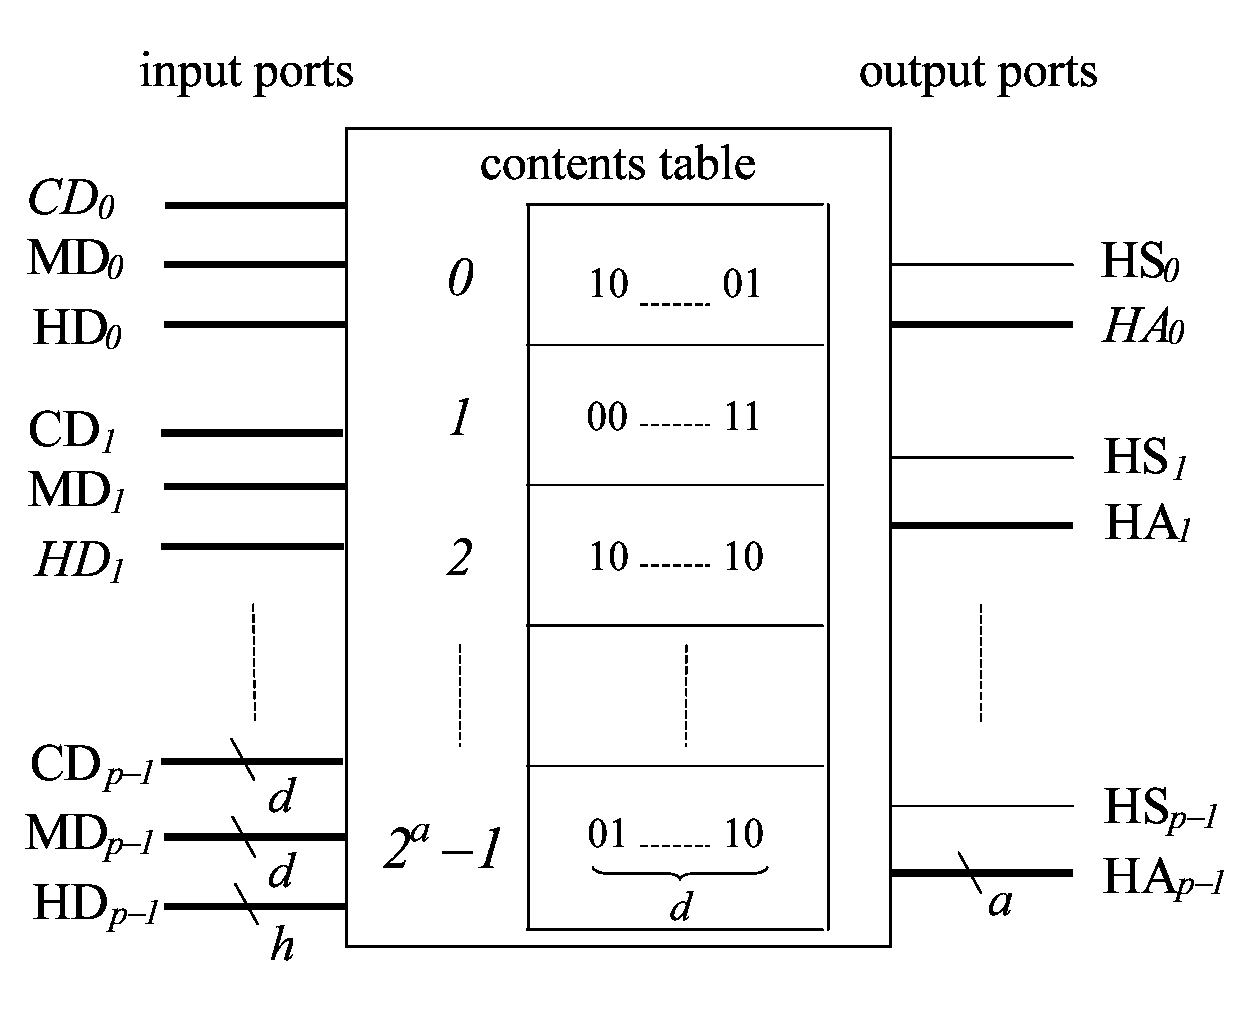
\includegraphics[width = 12cm,  height = 12cm, keepaspectratio, clip]{./pics/fmcam.eps}
		\end{center}
		\caption{ワード長$d$-bit,ワード数$2^a$のFMCAM.}
%		\ecaption{FMCAM with $d$ bits $\times$ $2^a$ words.}
		\label{fmcam}
	\end{figure}%	
%figure		

		\subsubsection{柔軟な検索機能}
		\label{fmcam_jyunan}
			FMCAMはマルチポートであり,ASIC及びFPGAに実装することで高い処理能力を得ることができ,
			マルチポートを生かした柔軟な検索機能を利用することが可能となる.そのため
			既存のCAMと比較して次に示すようなことが実現可能である.

			\begin{enumerate}
				\item 適用アプリケーションに合わせてポート数が変更可能

				FMCAMはデータを格納しているモジュールと,データの一致検索を行うモジュールが
				互いに独立しているため,ポート数の増減が容易に可能である.
				従って,適用するアプリケーションに応じて最適なポート数
				を持つように構成できるという特徴を有する.

				\item ポート毎に独立したマスクを指定可能

				FMCAMは,ポート毎に独立してマスクデータを設定することができるため,
				幅広い検索が可能となる.

				一例として,文献\cite{okuren, kazdou}等で提案されている最小値検索がある.
				これは,FMCAMの各ポートに長さの異なるマスクデータを用意したうえで,同一の比較データを
				入力することで一度にポート数分処理できるため,処理時間を短縮することができるようになる.

				\item あいまい検索

				文献\cite{chiint, ikesai, jalass}では,検索にハミング距離の概念を導入したCAMを提案している.すなわち
				``あいまいさ (approximate)''も含めて一致とするものである.
				これによって柔軟な検索を可能としているが,
				FMCAMは,ポート毎に独立してハミング距離を指定することを可能としている.そのため,より柔軟なあいまい検索が可能となる. 
				例えば,4つのポートに,各々ハミング距離を0 (通常の一致検索),1,2及び3と
				指定した場合,同一の比較データ``00000"を各ポートに入力しても,
				一致するものはそれぞれ``00000",``00100",``11000",``01011"などというように異なることとなる.
				\end{enumerate}

			\subsubsection{適用アプリケーション例}
			\label{fmcam_appli}
				FMCAMは,高い処理能力と柔軟な検索機能で様々なアプリケーションへ適用できる利点を持つ.
				本論文では,FMCAMをマルチメディアアプリケーションのボトルネックとなっている,
				テーブルルックアップ処理へ適用し,その有効性を検証する.
%				しているものにルーティング及びベクトル圧縮があり,その概要を述べる.
%
%				近年,ネットワークの高速化に伴い,従来のソフトウェアやメモリによるルーティングに代わって
%				CAMを内蔵するルータやスイッチが普及してきている.その中でも更なる性能向上を目指して
%				並列CAMを用いているものがあるが,コスト,ハードウェア量共に大きくなる傾向にある\cite{ccocis, hayfla}.
%				このようなルーティングにFMCAMを適用することで,高速性はそのままに,大幅なハードウェア量の削減及びコストの削減に
%				つながると考えられる.
%
				特にハフマン符号化は,
				テーブルルックアップ処理を利用する圧縮アルゴリズムとして知られており,
				近年のマルチメディアデータ処理の発展から,高効率の圧縮方法の1つとして注目を浴びてきている.
				これは文献\cite{hufmcm}にて提案された方式で,特に画像,音声及び動画等に向けた
				研究が盛んである.
%				ハフマン符号化圧縮関してはソフトウェアのみならずハードウェア化も試みられており,CAMを応用している
%				例もある\cite{kazdou}.
				FMCAMは,従来並列化が困難であったこのアプリケーションについても,
				高速に処理できる可能性を持っており,ハードウェア量及びコストの削減に
				つながるものと考えている.
				特にハードウェア量を小さくすることは,携帯端末等への応用につながるものと考えられる.



\subsection{アーキテクチャ}
\label{lbl_cp4_fmcam_architecture}

%\subsubsection{内部構成}
%\label{lbl_cp4_fmcam_kousei}

		FMCAMは,
		マルチポート化,比較対象データのカテゴリ分け処理,及び比較データの即時処理に特化した
		構成をとっている.

		図 \ref{fmcam_block}に,内部構成のブロック図を示す.FMCAMは大きく分けて4つのモジュール,
		すなわち``カテゴリモジュール (CaM)'',
		``コンテンツモジュール (CoM)'',``セレクタモジュール (SeM)''及び``ポートモジュール (PoM)''
		から構成されている.

%figure
	\begin{figure*}[tbh]
		\begin{center}
			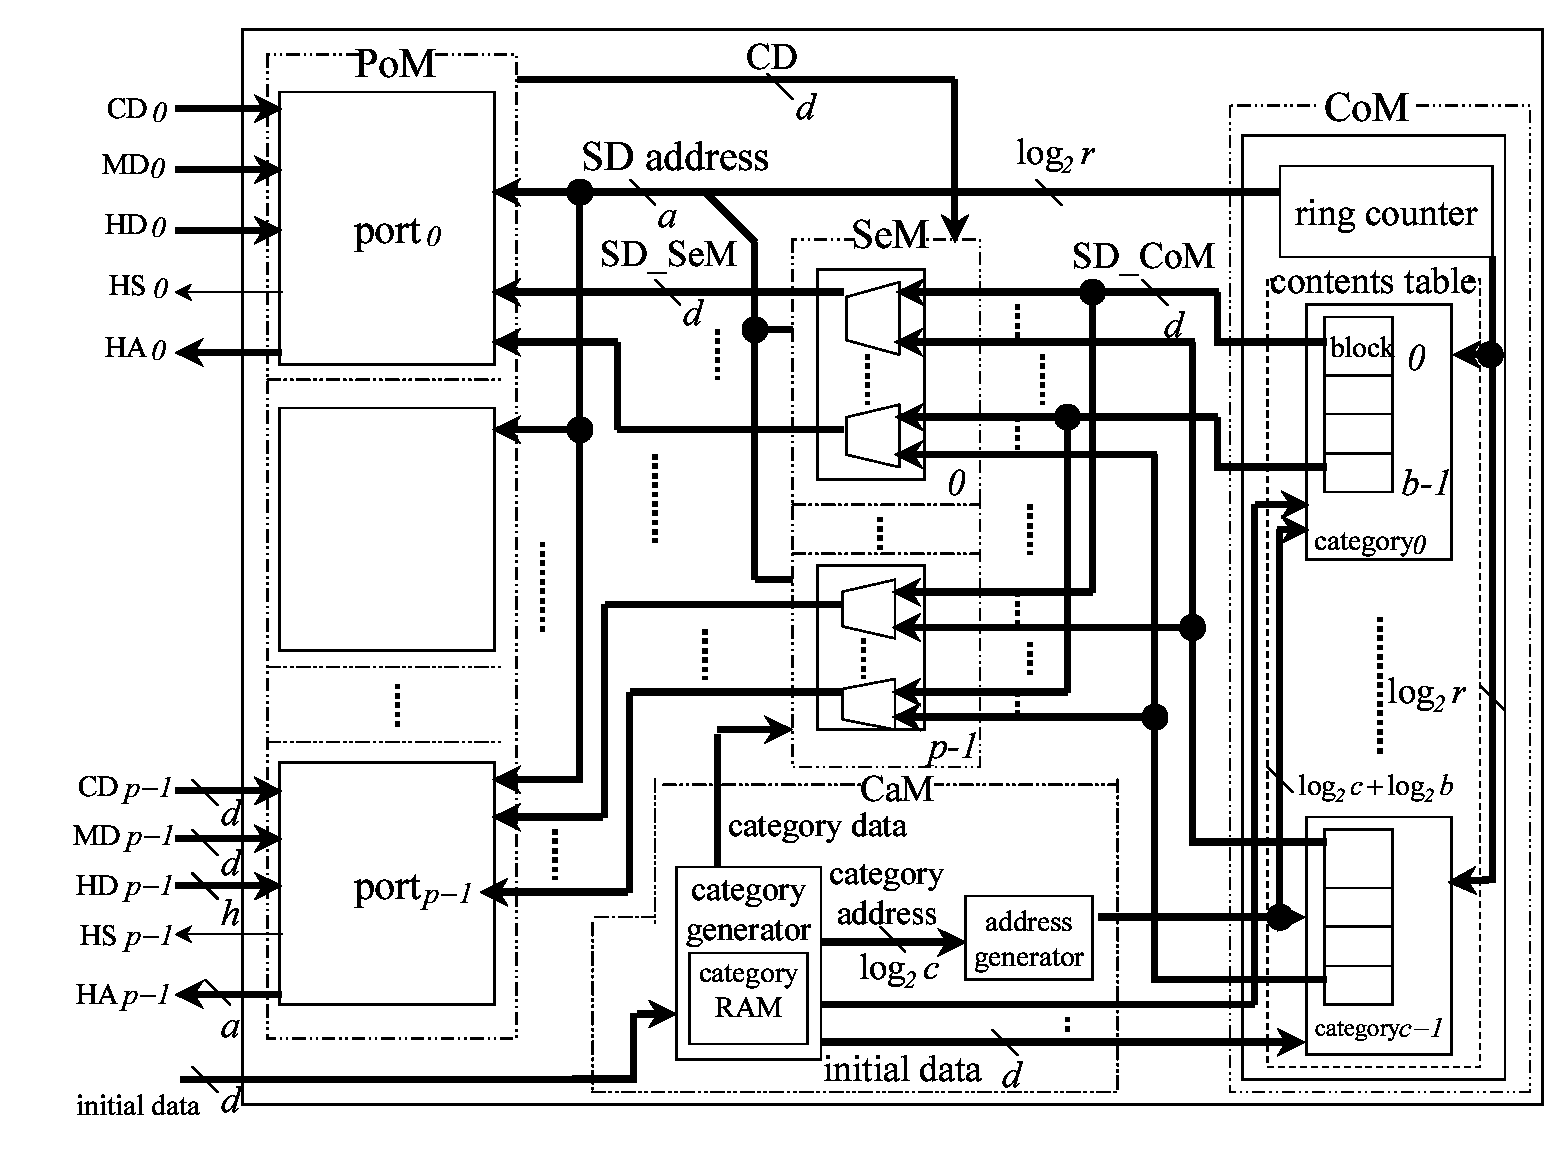
\includegraphics[width = 14cm,  height = 14cm, keepaspectratio, clip]{./pics/fmcam_block.eps}
		\end{center}
		\caption{FMCAMの内部構成.}
%		\ecaption{Block diagram of FMCAM.}
		\label{fmcam_block}
	\end{figure*}%	
%figure

	\begin{enumerate}
		\item カテゴリモジュール

			内部にはカテゴリRAMを内蔵したカテゴリジェネレータとアドレスジェネレータが格納されている.
			カテゴリジェネレータ及びカテゴリRAMは,初期化の際に外部からデータを受け取って\ref{cat_syori}節にて詳述する
			カテゴリ分けのための処理を行う.
			またアドレスジェネレータは,この外部からのデータをコンテンツテーブルに格納するためのアドレスを,カテゴリに基づいて
			生成し,コンテンツテーブルへと送出する.

			
	\item コンテンツモジュール

			このモジュールは,図 \ref{fmcam_block}に示すカテゴリを$c$個ひとまとめにしたコンテンツテーブル,及び
			\ref{ring}節にて詳述するリングカウンタ を格納するモジュールである.

			FMCAMはBPBP (Bit-Parallel Block-Parallel)方式を採用しており,図 \ref{byt_ram}に示すように1ブロックは$d$-bit長の比較対象データ (SD\_CoM)を
			$r$ワード格納しているため,リングカウンタは0から$r - 1$までのアドレスを1クロックサイクル毎に順次出力することになる.
			よって各ブロックからは全データを$r$クロックサイクルで読み出すことができ,
			FMCAMは,全ての一致検索処理を$r$クロックサイクルで完了できる.
 
			1カテゴリは,ブロック$b$個分に相当しており,コンテンツテーブルにはカテゴリを$c$個用意してある.
			従って全ての比較対象ワード数は$2^a = cbr$と表すことができる.初期化の際には,
			 ライトイネーブル信号,外部からの初期データ及びそのアドレスが送られてきて,
			各カテゴリに格納される.

%figure
	\begin{figure}[tbh]
		\begin{center}
			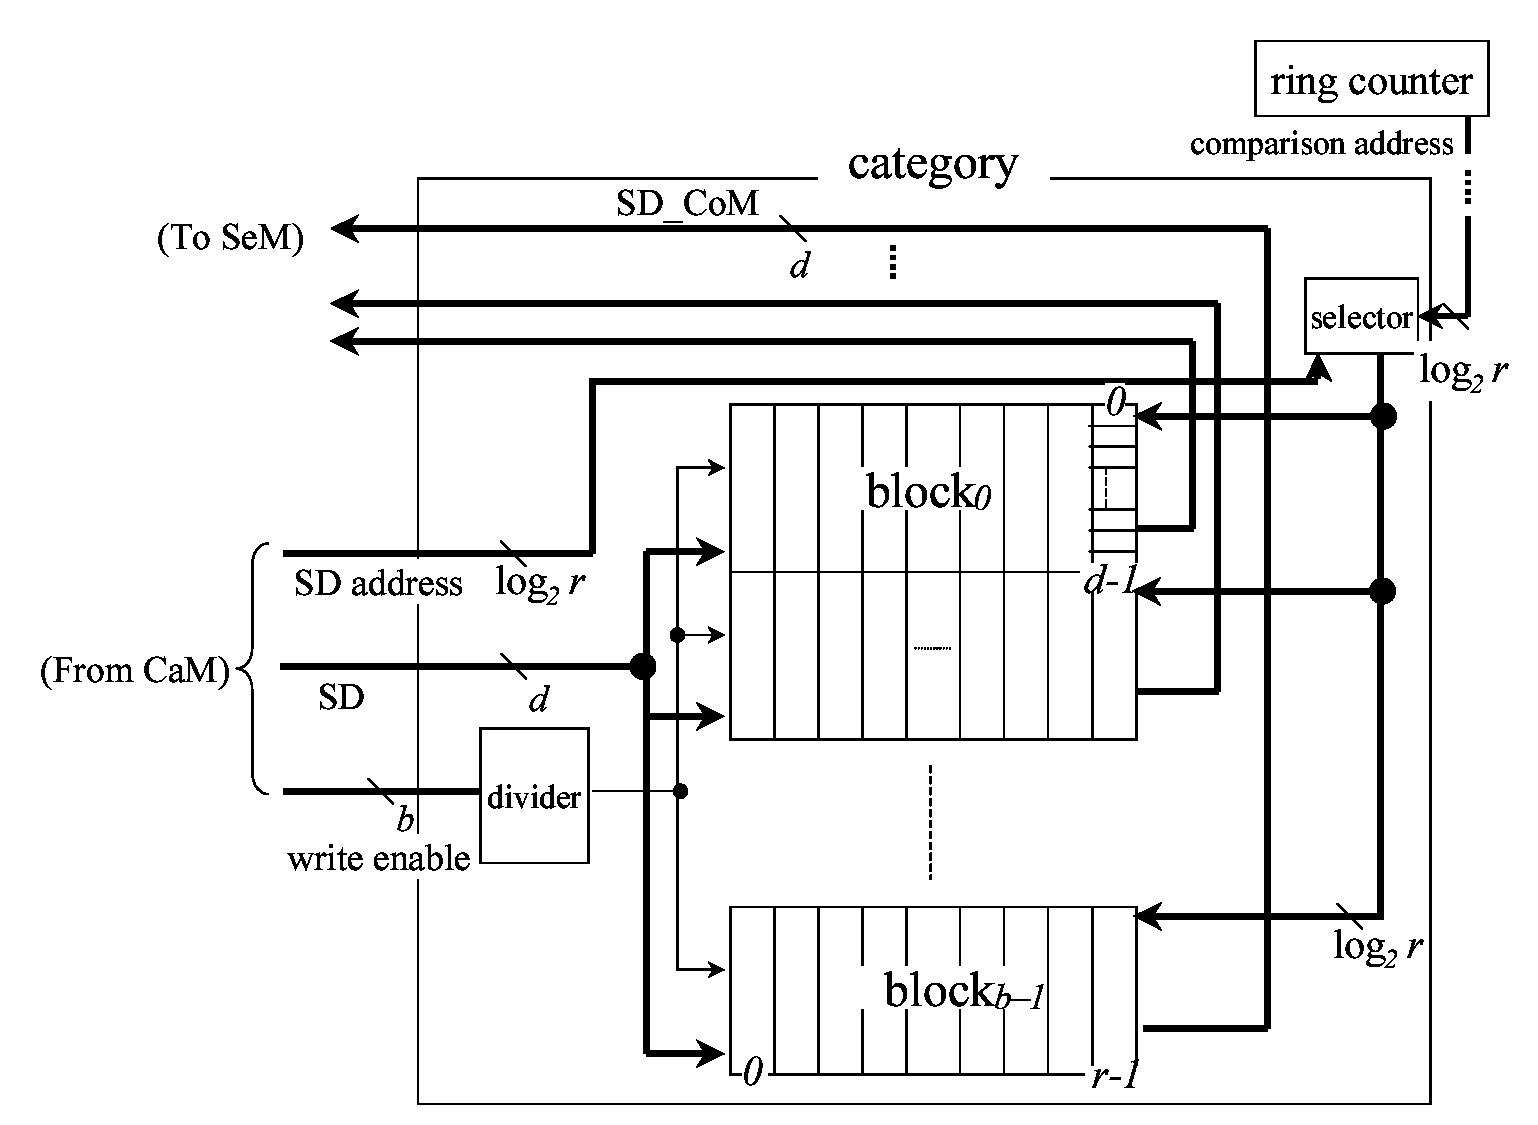
\includegraphics[width = 14cm,  height = 14cm, keepaspectratio, clip]{./pics/byt_ram.eps}
		\end{center}
	\caption{コンテンツモジュール (CoM)内のカテゴリ.}
%		\ecaption{Block diagram of a category in a CoM.}
		\label{byt_ram}


	\end{figure}%	
%figure

		\item セレクタモジュール

			このモジュールは,各ポートモジュールに対応させてポート数分用意されている.図 \ref{mux}に示すように,
			このモジュールの内部には,カテゴリセレクタと$c$対1のマルチプレクサが$b$個用意されている.
			カテゴリセレクタは,比較データ (CD)から対応するカテゴリを判別し,
			各マルチプレクサに選択信号を送信する.この信号を受けてマルチプレクサは,$c$個の
			比較対象データ (SD\_CoM)のうち対応するカテゴリのデータを選択して,ポートモジュールへ対応する
			比較対象データ (SD\_SeM)を送出することになる.

%figure 
	\begin{figure}[tbh]
		\begin{center}
			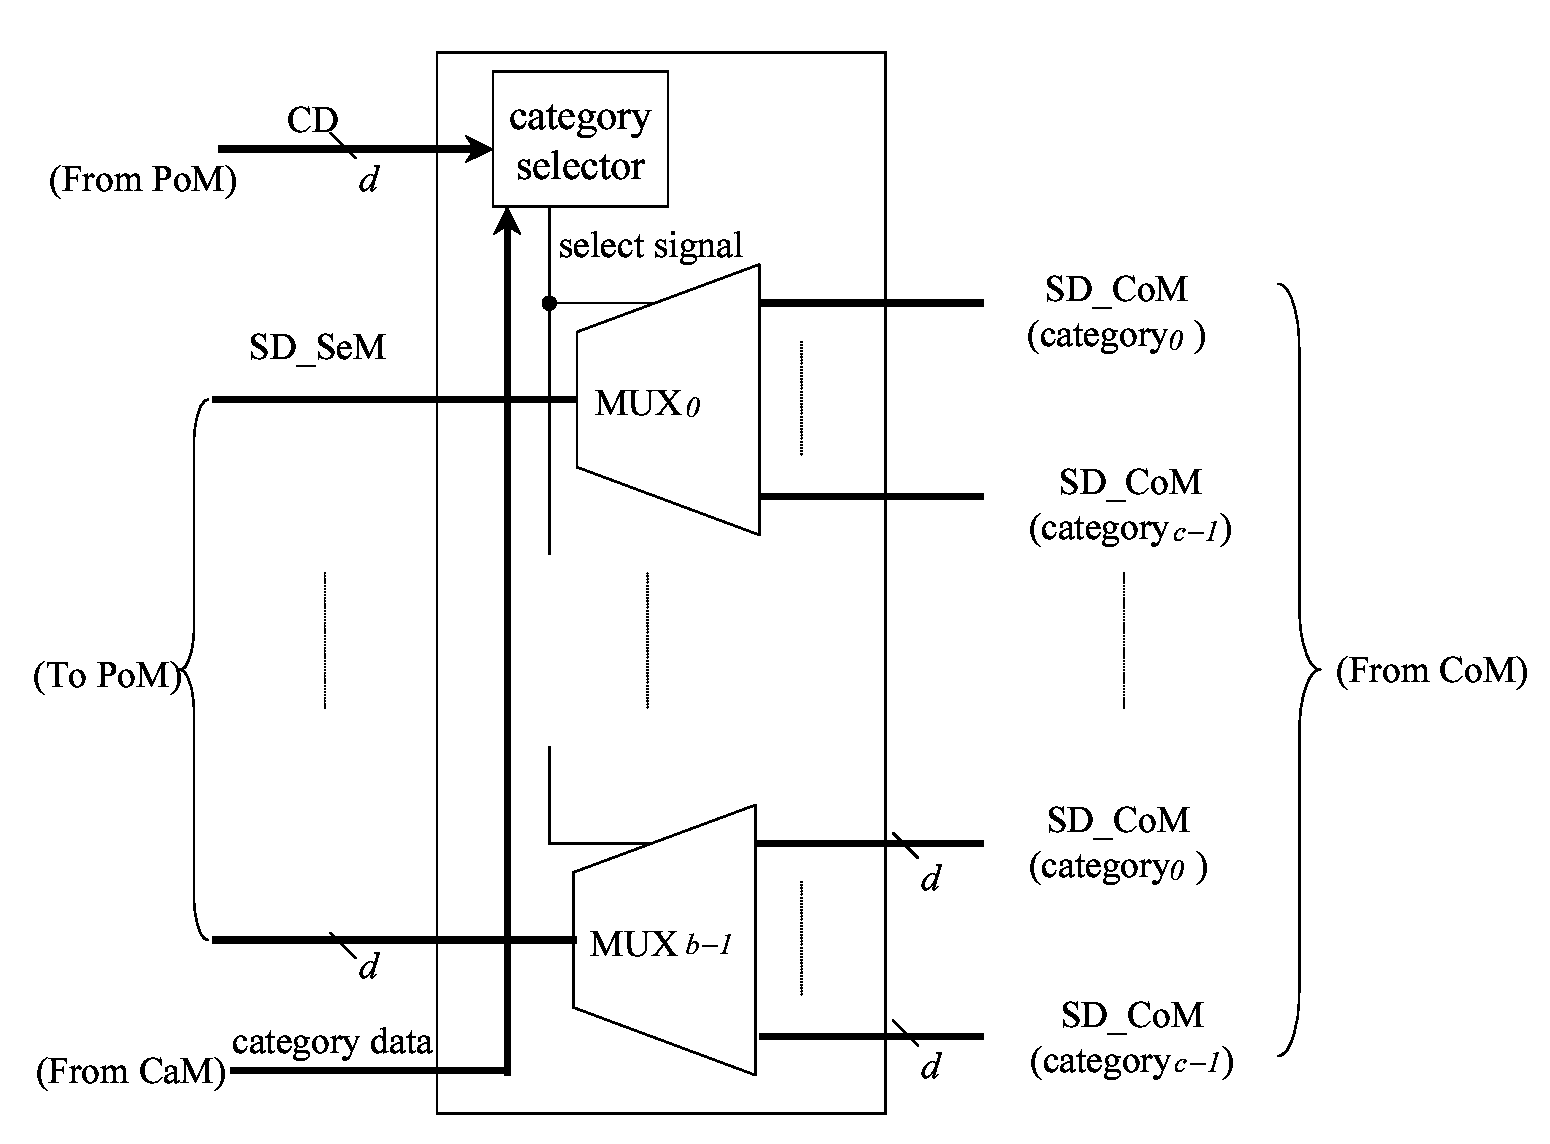
\includegraphics[width = 14cm,  height = 14cm, keepaspectratio, clip]{./pics/mux.eps}
		\end{center}
		\caption{セレクタモジュール (SeM).}
%		\ecaption{Block diagram of a Selector Module.}
		\label{mux}
	\end{figure}%	
%figure

		\item ポートモジュール

			データの入出力を行うモジュールであり,FMCAMはこのポートモジュールをポート数分持つ.
			図 \ref{prt_module}にポートモジュールのブロック図を示す.比較データ (CD)を受け取ったポートモジュールは,
			まずセレクタモジュールへこのデータを送信する.
			その後,セレクタモジュールから対応する比較対象データ (SD\_SeM)が比較器に送られてくるので,ポートモジュールで受け取った
			比較データと比較処理される.なお,比較データと同時に入力されるマスクデータ (MD)の対応ビットが1になっているビットについては,
			比較結果を反映させないことでマスクしている.また,ハミング距離 (HD)が指定されている場合には,プライオリティエンコーダに
			比較結果を送信する前に,ファンクション回路であいまい検索等の処理を行う.
			なお,このプライオリティエンコーダは,複数のヒットがあった場合に優先順位の高い比較対象データを選択し,
			一致信号 (HS)とそのアドレス (HA)を出力するためのものである.
			また,コンテンツテーブル内の各カテゴリは$b$個のブロックに分割されているため,
			比較器もそれに応じ$b$個用意されている.
			ここで示したポートモジュールは互いに独立しており,再構成によってその数も増減可能である
			ため,適用アプリケーション毎に必要なポート数を柔軟に確保することが可能となる.

	\end{enumerate}
%figure
	\begin{figure}[tbh]
		\begin{center}
			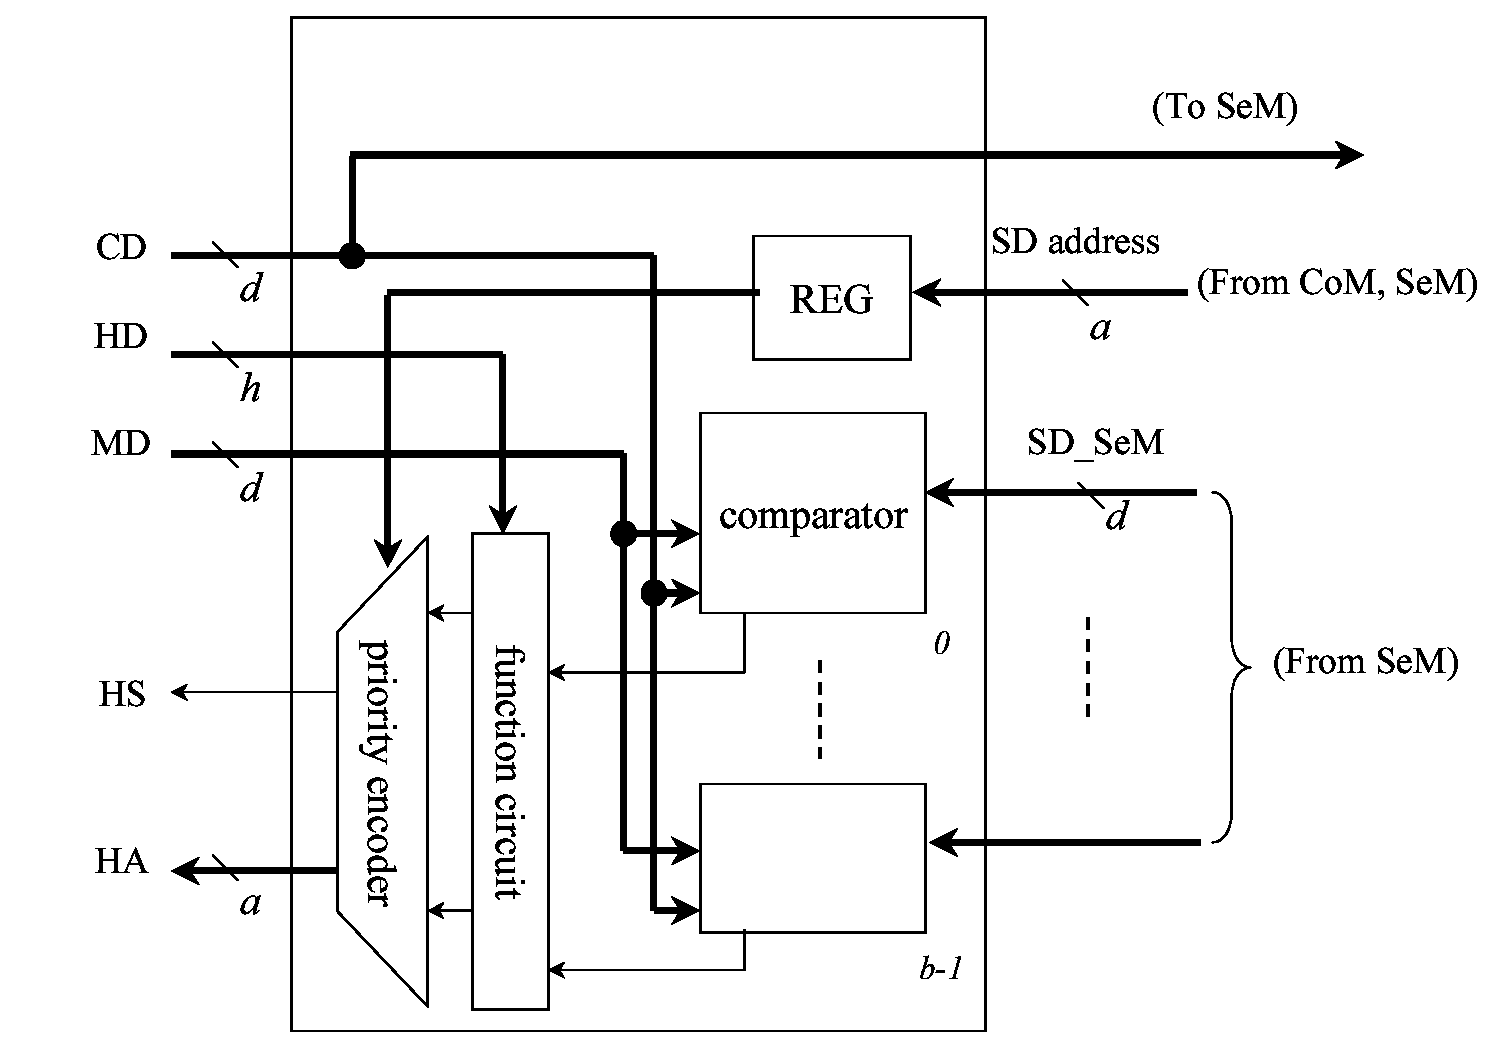
\includegraphics[width = 14cm,  height = 14cm, keepaspectratio, clip]{./pics/prt_module.eps}
		\end{center}
		\caption{ポートモジュール (PoM).}
%		\ecaption{Block diagram of a Port Module.}
		\label{prt_module}
	\end{figure}%	
%figure

\subsection{マルチポートの実現方法}
\label{fmcam_tokutyo}
	CAMにとって,処理速度の向上と大容量のコンテンツテーブルを両立させることは大きな課題であり,
	そのためにFMCAMはマルチポートでありながら比較器数の増大を抑えている.
	これを実現するための改良点の中で特徴的なものは,カテゴリ分け処理及び比較データの即時処理であり,それらの詳細を
	次に述べる. 
	\subsubsection{カテゴリ分け処理}
	\label{cat_syori}
		
			\ref{lbl_cp4_cam_mondai}節のマルチポート化の課題1で述べた問題を解決するために,比較器の位置を従来のコンテンツテーブル付近から
			ポートモジュールへ移動することを考案した.
			そのため,この2つのモジュールの中間にセレクタを配し,
			カテゴリ分けされた比較対象データの中から対応するもののみをポートモジュール内で比較できるようにしている.

			FMCAMは,初期化時に入力される外部からのデータを内部のコンテンツテーブルに書き込む段階で
			カテゴリ分けを実行し, 
			カテゴリは,そのデータの上位ビットから判定するものとしている.
			図 \ref{fmcam_block}に示したカテゴリモジュール内では,あらかじめ指定したカテゴリの値を
			カテゴリRAM内に記憶させておき,
			入力された比較対象データに基づいてカテゴリジェネレータが対応するカテゴリを決定する.
			 
			このカテゴリに基づいて,外部からのデータは対応するコンテンツテーブル内のカテゴリに格納される.
			FMCAMは,このカテゴリ分けを初期化の段階で実行し,外部から入力される全てのデータに対してカテゴリ分けの処理が終了
			した時点で,一致検索の準備が完了したこととなる.
 
			カテゴリ分け処理による一致検索は,まず任意のポートモジュールが比較データを受け取ったならば,対応するセレクタ
			モジュール内のカテゴリセレクタへ比較データを送出する.
			カテゴリセレクタは,初期化の際にカテゴリモジュールからカテゴリデータを
			受け取り,そのデータを保持しているため,比較データを受け取ったならば,その上位ビットから
			カテゴリを判断できる.そしてマルチプレクサが,コンテンツモジュールから順次ブロードキャストされてくる比較対象データの中から適する
			ものを選択し,ポートモジュールへと送信する.
			その後に,ポートモジュールで一致検索が開始されることとなる.
			この結果,各ポートモジュールで一致検索を並列に行なえるようになったため,
			コンテンツテーブルの近傍に位置している比較器をポートモジュール固有のものとし,
			その数を大幅に削減できた.


	\subsubsection{比較データの即時処理}
	\label{ring}

		\ref{lbl_cp4_cam_mondai}節のマルチポート化の課題2で示した問題を解決するため,
		新たな機構としてリングカウンタを通常のアドレスカウンタの代わりに採用した.
		リングカウンタは,コンテンツテーブルの初期化が終了した後,入力データの到着に関わらず
		常時ループカウントし続けることとした.
		なお,1サイクルのカウント数はブロック内のワード数である$r$で決まるため,0から$r - 1$となる. 
	
		図 \ref{ring_cnt}に示すように,ある時点においてポート0と$p - 1$に比較データCD$_0$及びCD$_{p - 1}$が到着したならば,
		その時点のアドレス$a_i$をそれらのポートモジュール内の
		レジスタに保持することで検索開始アドレスを記憶した後,比較処理を開始する.その後ポートモジュールには逐次アドレスが,
		$a_{i+1}$, $a_{i+2}$, $\cdots$ $a_{r-1}$, $a_0$, $a_1$, $\cdots$, $a_{i-1}$
		と送られてくるので,次の$a_i$が来たならばアドレスが一巡したこととなるため,一連の比較処理を終了する.
		このようにして,コンテンツテーブル内の対応するカテゴリの比較対象データ全ての検索を
		行うことが可能となる.
		ポート0及び$p - 1$の比較処理中に,ポート1に比較データCD$_1$が到着した
		場合でも,その時点の処理開始アドレス$a_j$をポートモジュール1内のレジスタに保持
		することで待ち時間を必要とせず,ポート1も比較処理を即座に開始できる.

		このようなリングカウンタの適用で,並列CAMを用いなくとも,FMCAM単体で同様の処理を行なえるようになった.

%figure
%		\vspace{3mm}
	\begin{figure}[tbh]
		\begin{center}
			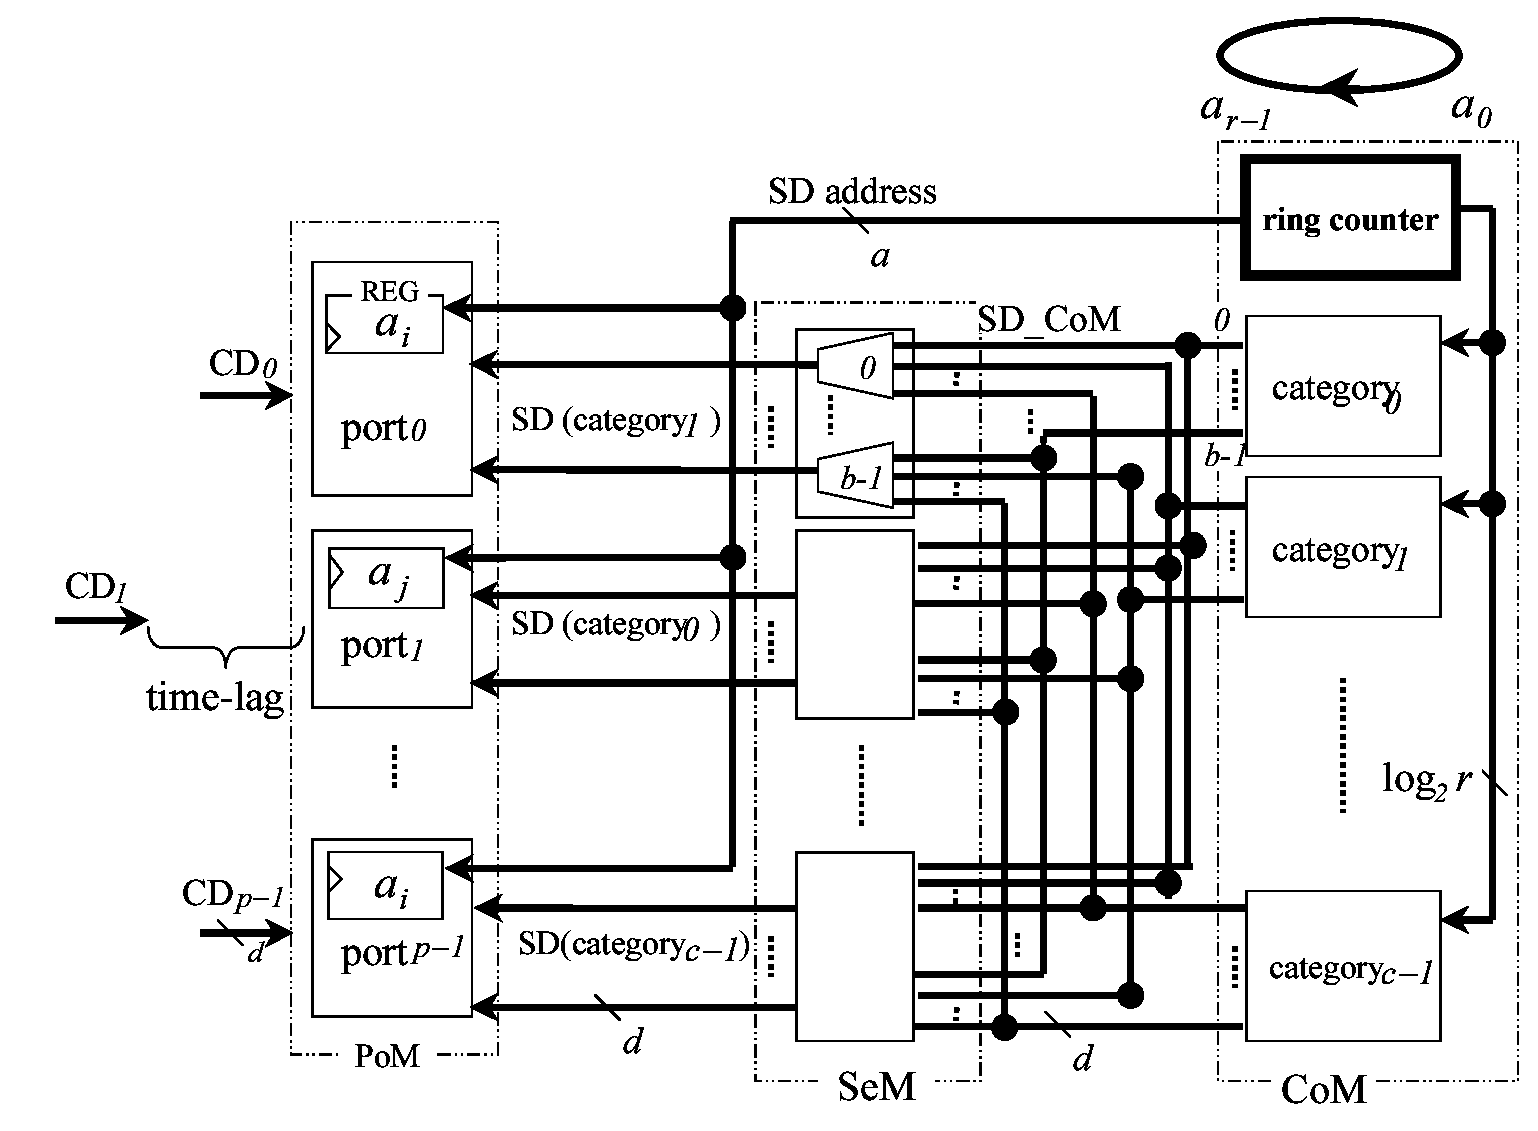
\includegraphics[width = 14cm,  height = 14cm, keepaspectratio, clip]{./pics/ring_cnt.eps}
		\end{center}
		\caption{リングカウンタを用いた比較方式.}
%		\ecaption{Comparison process with a ring counter.}
		\label{ring_cnt}
	\end{figure}%	
%figure


\subsection{FPGAへの実装結果}
\label{lbl_cp4_fmcam_hyouka}

		本節では,提案したFMCAMをXilinx社製FPGAであるXC2V6000に実装した.
		図 \ref{kac02a}に使用した,FPGAボードである三菱電機エンジニアリング製KAC-02Aの写真を示す.
		ボード上には,XC2V6000が2石搭載してあり,PCIバスを経由してホストコンピュータとデータのやり取りを行う.
		また,設計はVerilog-HDLを使用し,設計ツールはXilinx社のISE Foundation 4.2i,
		論理合成にはXST Verilogを用いた.

%figure
\begin{table}[tbh]
%		\vspace{-4mm}
		\caption{実装に用いたFPGAボード.}
%		\ecaption{Implementation results of FMCAM.}
%		\vspace{-3mm}
			\begin{center}
				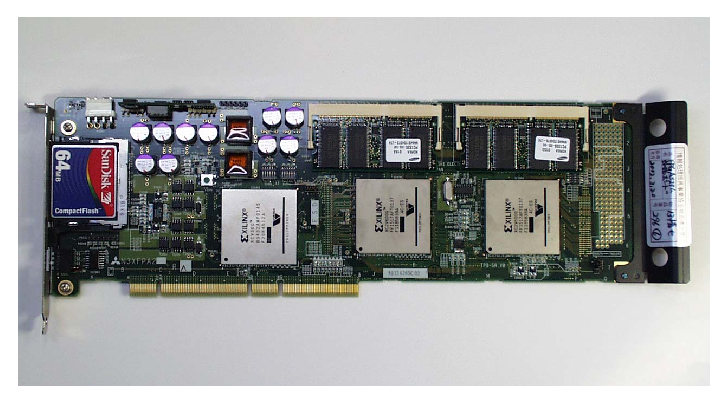
\includegraphics[width = 14cm,  height = 14cm,  keepaspectratio,  clip]{./pics/kac02a.eps}
			\end{center}
		\label{kac02a}
%		\vspace{-10mm}
	\end{table}%


	\begin{table}[tbh]
%		\vspace{-4mm}
		\caption{FMCAMのFPGAへの実装結果.}
%		\ecaption{Implementation results of FMCAM.}
%		\vspace{-3mm}
			\begin{center}
				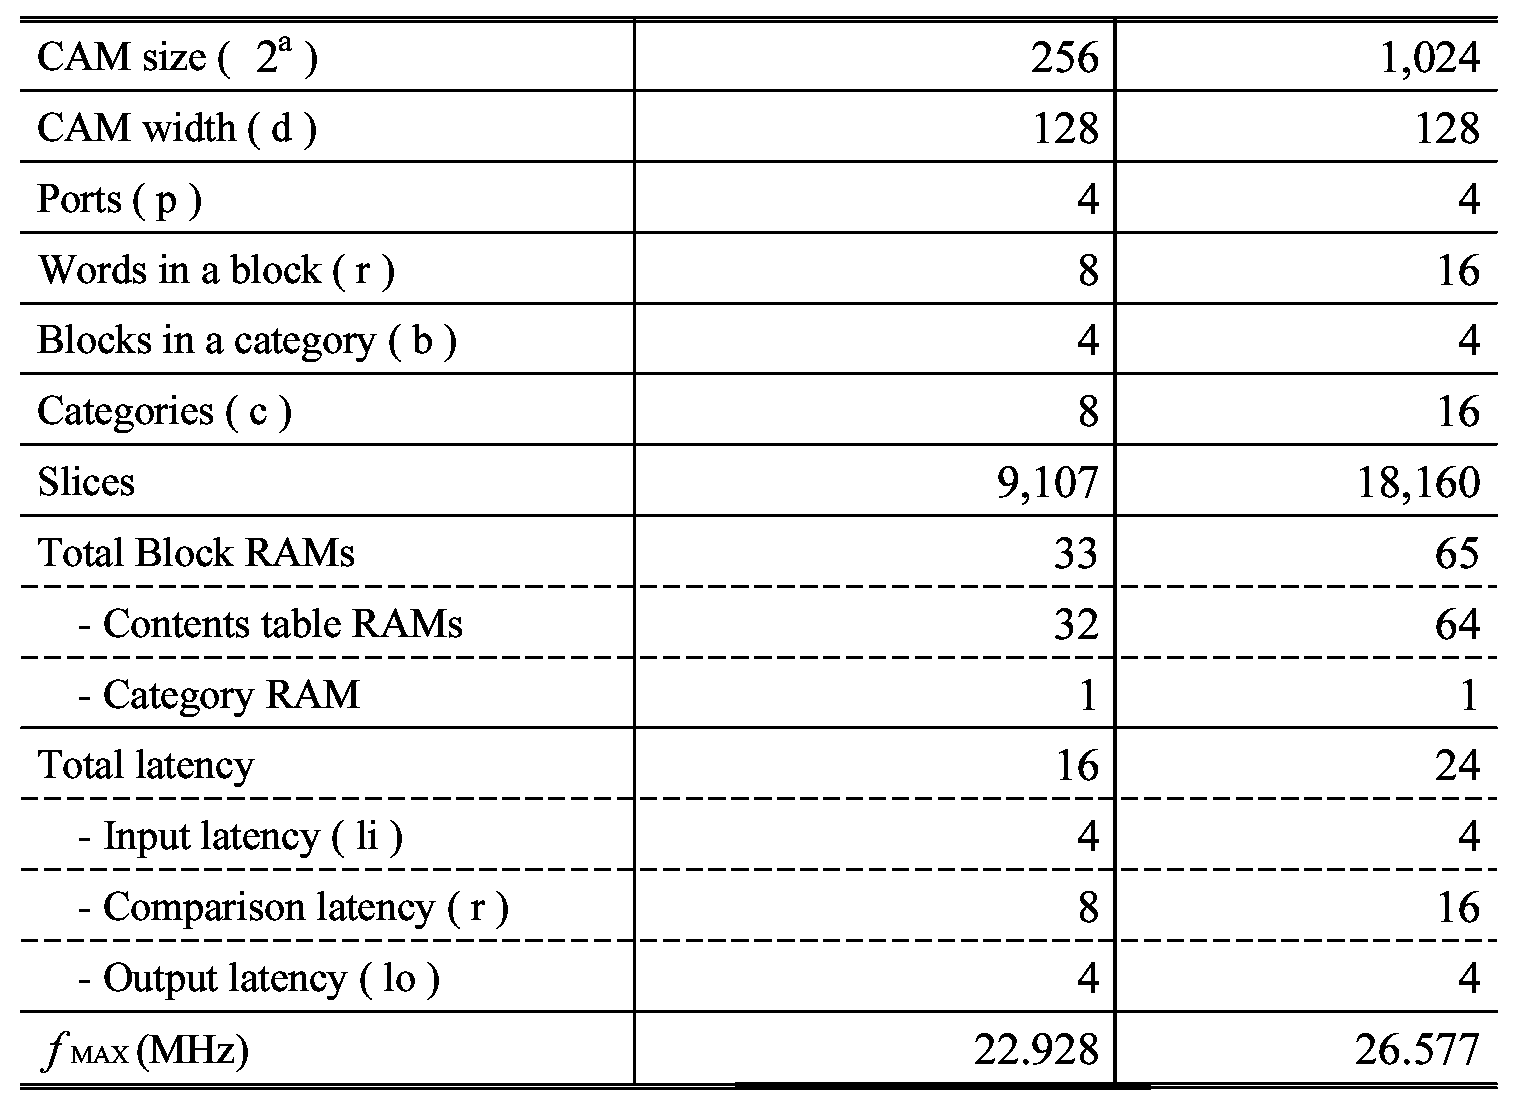
\includegraphics[width = 12cm,  height = 12cm,  keepaspectratio,  clip]{./pics/data.eps}
			\end{center}
		\label{data}
%		\vspace{-10mm}
	\end{table}%

		表 \ref{data}に設計したFMCAMの諸元及び実装結果を示す.
		今回は,ワード数$2^a$の変化に伴う実装結果の違いを確認するため,この値を256及び1,024と異なる2種類のFMCAMを開発した.
		ただし,ワード長$d$はどちらも128 bitである.また,RAM及びレイテンシに関してはそれぞれ内訳を破線にて示している.



\begin{enumerate}
	\item ハードウェア量

		ワード数1,024のFMCAMは,ワード数256のものと比較して,コンテンツテーブルの容量が4倍になっている.
		このとき,既存の方式のCAMでは,比較器も元の4倍必要となる.
		しかし,FMCAMは比較器をコンテンツテーブルと独立させてポートモジュールに配置しているため,
		ワード数の増加に対して比較器数は変化しない.
		増加したリソースは,主にコンテンツテーブルの容量を増加させるための増加分及び
		コンテンツテーブルからセレクタモジュールへのバスエリアである.
		結果としてFMCAMは,比較器数のFPGAの基本ロジックであるスライス数による比較では1.99倍程度の増加にとどまった.
		このようにFMCAMは,コンテンツテーブルを拡大させたにも関わらず,
		ハードウェア量の増加を少なく抑えられていることが確認できた.


	\item 処理性能
	\label{sokudo}

		FMCAMのレイテンシは,入力データが確定してから,出力データが確定されるまでの
		クロックサイクル数で測定したものである.
		比較にかかるクロックサイクル数 (Comparison latency)が,
		ワード数によって差異があるが,これはBPBP方式の特性によるものであり,
		ブロック内のワード数$r$が8及び16と異なるためである.
		
		 動作周波数に関しては,回路規模が小さいワード数256のものが回路規模の大きい1,024のものより
		通常高くなると考えられるが,今回の実装結果では反対になっている.
		この理由としては,使用したFPGAであるXC2V6000が大規模回路設計向けのものであることが考えられる.
		XC2V6000の全体の使用可能スライス数は33,792であり,	これより各FMCAMの使用スライスの割合は1,024のものが54\%,
		256のものが27\%となる.よって256のものは外部ピンから内部のレジスタまでのパスやその他の
		レジスタ間のパスが1,024のものと比較して長くなるため動作周波数は低くなったものと考えられる.
\end{enumerate}


 \subsection{性能評価}
\label{lbl_cp4_fmcam_hyouka}
		FMCAMの性能を評価するために,比較方式及び既存のCAMとの比較検討を行なった.
		尚ここでは,幅広い観点から評価を行うために,ASIC,FPGA及び並列CAMを評価対象としている.

\begin{enumerate}
	\item CAMの比較方式による性能評価
\label{hard_kousei}

	ここでは,各方式のCAMの性能を,比較器数と比較にかかるクロックサイクル数の両面から
	評価してみることにする.

			FMCAMとBSWP (Bit-Serial Word-Parallel)方式 \cite{kobbit},BPWP方式,BPBP方式及びカテゴリ分けを行うCAM,それぞれの比較器数の
			算出式$N$は,表 \ref{noc}の様になる.
%table
	\begin{table}[tbh]
		\caption{構成方法による比較器数及びクロックサイクル数.}
%		\ecaption{Number of comparators and clock cycles.}
			\begin{center}
				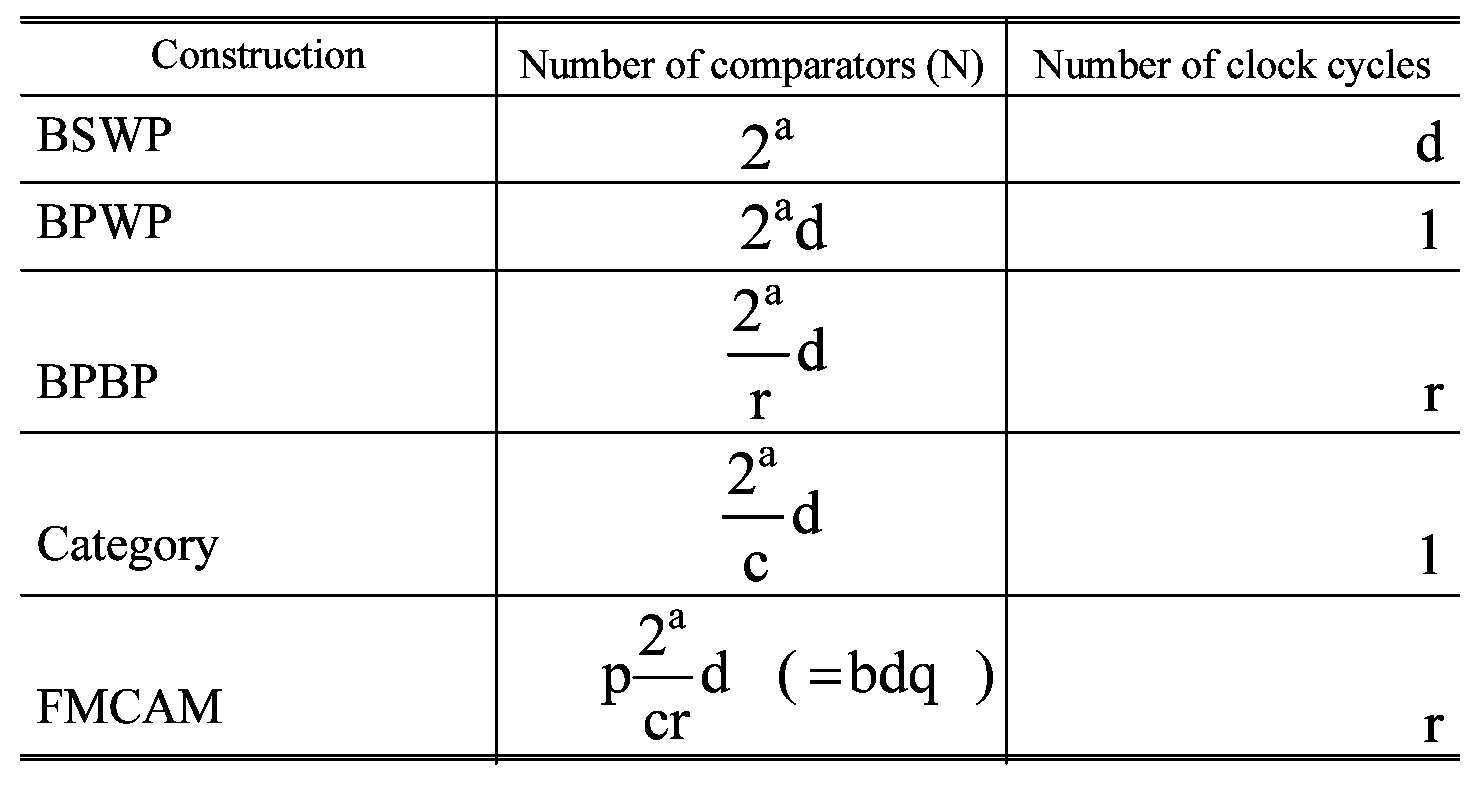
\includegraphics[width = 12cm,  height = 12cm, keepaspectratio, clip]{./pics/noc.eps}
			\end{center}
		\label{noc}
	\end{table}%

			ここで,$a$はコンテンツテーブルのアドレスのビット幅,$d$は比較データのビット幅,$c$はカテゴリの個数,
			$b$は1カテゴリ内のブロックの個数,$r$は1ブロック内の比較対象データの個数,そして$p$はポート数である. 			
			各式の全体的傾向として,いずれの$N$も$2^a$に比例しているため,$a$の増加に対して指数関数的に増加することになる.

			BSWP方式においては,
			$N$の値に$d$を乗じないため,他の$N$と比べて最も小さいが,
			比較に要するクロックサイクル数が$d$となるため比較処理に多くの時間を要する.
			BPWP方式の比較にかかるクロックサイクル数は1であり最も高速であるが,
			他の式と比べて最も$N$の増加が著しいものとなる.
			よってこれらの方式は,適用アプリケーションに対して制限が大きいものといえる.

			BPBP方式及びカテゴリ分け方式においては,
			$r$もしくは$c$で除された分,$N$の増加が抑えられていることが分かる.
			しかし,BPBP方式は$r$を過度に増やすと比較速度は低下し,
			カテゴリ分けを行うCAMでは一般的にBPWP方式を用いているので,比較にかかるクロックサイクル数が1ではあるが,
			カテゴリ分けのための機構が別に必要となり,この処理に数クロックかかる.また,
			$c$の値は適用するアプリケーションに依存することが多い.	

			FMCAMにおいては,
			$r$および$c$の積で除されて
			$N$の値が抑えられるため,比較器数を大幅に削減することが可能となっている.
			また比較器をコンテンツテーブルから独立させているため,$p$は$2^a$に対して独立変数であり,
			$2^a$や$cr$の値に対して高々僅かであるため,
			それを乗ずることによっても比較器の増加数は僅かで済む.
			FMCAMは,BPBP方式とカテゴリ分けのデメリットを抱えることにはなるが,
			マルチポート化しているため処理能力が高く,このデメリットを凌駕すると考えられる.
 			以上よりFMCAMは,
			マルチポート化により処理能力を向上しつつ,
			それに伴う比較器数の増加を大幅に抑えている.またコンテンツテーブルが拡大しても,
			比較器数がそれほど増加しないように抑制することに成功している.


	\item 既存のCAMとの比較
	\label{cam_hikaku}

	FMCAMを含めた各CAMの諸元,対象LSI及び比較方式を表 \ref{atp_comb}に示す.
		比較対象のCAMとしては,各ベンダから現在リリースされている標準的なCAMを選択した.
		これらのうちFPGAをベースとしたものとしては,次の3種類を選択した.Xilinx社のアプリケーションノートで公開されているXAPP CAMのうち,
		BPBP方式であり大規模用途向けのXAPP202 \cite{defcon},BPWP方式であり小型で高速なXAPP 203\cite{bredes},
		そしてALTERA社からFPGA内に組み込み済みの専用CAMのAPEX CAM\cite{camalt}である.
		またASICとしては,IPv6ルーティング向けの大規模高速なCAMであるミュージックセミコンダクタ社のLANCAM MP\cite{mu9mus}を選択した.

%table
	\begin{table}[tbh]
		\caption{各種CAMのスペック及びAT積.}
%		\ecaption{Specification and AT products of CAMs.}
			\begin{center}
				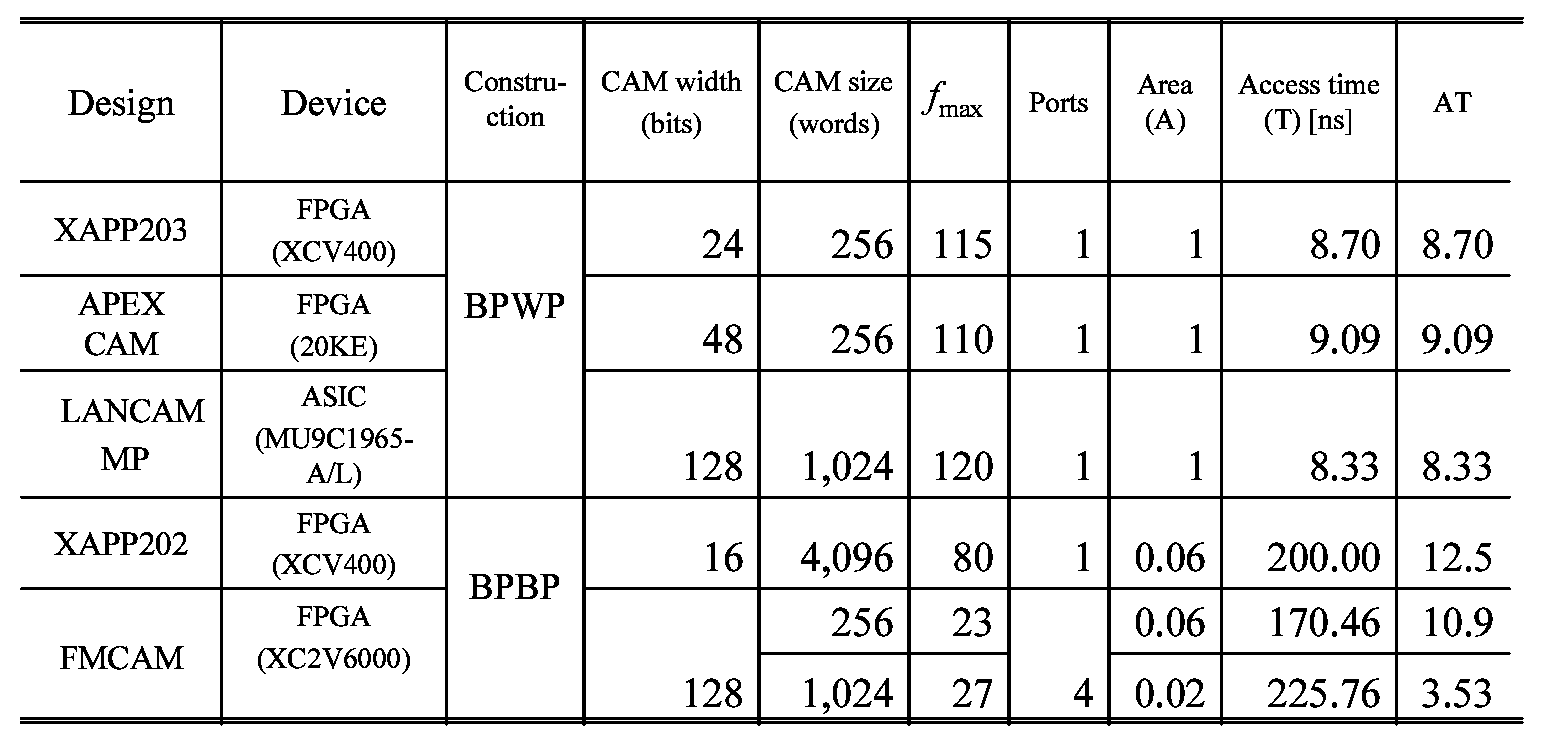
\includegraphics[width = 14cm,  height = 14cm, keepaspectratio, clip]{./pics/atp_comb.eps}
			\end{center}
		\label{atp_comb}
	\end{table}%
%table 

		評価方法として,CAM自体の総合的な性能をAT (Area-Time)積で表したものが
		文献\cite{hardet}で示されており,本論文ではこれを用いて既存のCAMとFMCAMの性能比較を行なった.
		以下にその算出式を示す.なお,各変数は表 \ref{data}に使われているものとなっている.
			
\begin{equation}
	AT =
		\frac{N}{2^ad}
		\times 
		\frac{r + li + lo}{pf_\mathrm{MAX}}
		\label{eq_atp}
\end{equation}

			一般にAT積は回路規模と処理時間の積であり,この値が小さいほど優れている実装であるということが言える.
			この式を用いて様々な実装形態のCAMを比較するため,使用するチップの面積に相当するエリア (A)として
			比較対象ワード数を比較器数で正規化したものを用い,
			一方動作周波数と一致検索に必要なクロックサイクル数から算出された1ポートあたりのアクセスタイム (T)を処理に要する時間として,
			両者の積 (AT)を求めたものである.
			なお,正規化に関しては,実際にCAMのハードウェア量のうち,特に比較器の数がボトルネックとなっているという背景
			を考慮したものとなっている.
			これらのAT積を算出した結果も表 \ref{atp_comb}に併せて示す.

			まずエリアの値に関しては,BPWP方式の場合,全比較対象データの各ビットに
			比較器を持っているため全て1となる.これに対してBPBP方式では,比較器数を削減できるため,
			XAPP202及びワード数256のFMCAMの場合に0.06,ワード数1,024のFMCAMの場合に0.02とそれぞれ低い値を示していることが分かる.
			特にFMCAMは,比較器がコンテンツテーブルから独立してポートモジュールに配置してあるので,コンテンツテーブルの容量を4倍に拡大しても,
			直接影響は受けず,比較器数に変化はない.
			そのため今回の設計では,ワード数が異なる2種類のFMCAMの$N$の値は同値となり,エリア値はワード数1,024のほうが
			低い値を示している.

			アクセスタイムに関しては,BPBP方式の場合,BPWP方式の値と比較してどれも高い値にならざるを得ない.
			また,今回作成した2種類のFMCAMは,遅延パスの改善等配置配線時の制約条件がほぼ初期設定であるため,動作周波数は既存のものと比較して
			低いものとなっている.しかし,マルチポート化されており複数の処理を並列に実行できるので,
			アクセスタイムを算出する際,ポート数$p$で除することができる.そのためアクセスタイムがある程度抑えられる.

			このようにして算出された
			AT積を各CAMで比較すると,ワード数1,024のFMCAMが,最も良い結果を示していることが分かった.
			また,ワード数256のFMCAMは,同じBPBP方式のXAPP202より優れた値を出しているものの,BPWP方式のCAMと比較すると
			劣っていることが分かる.
			この結果よりFMCAMは,ワード数を大きくするほどAT積が低くなり,有利となる事が分かった.
			これは,カテゴリ分け処理によって比較器の数を徹底して削減しているため,コンテンツテーブルの拡大に対して
			比較器の数の増加が抑えられていることが反映したためである.



	\item マルチポートCAM及び並列CAMとの比較
	\label{para_cam_hikaku}

			FMCAMにおけるカテゴリ分けによる比較器の数の削減効果を詳しく検証するため,並列CAMと
			FMCAMからカテゴリモジュール,セレクタモジュール及びリングカウンタ等の機構を取り除き,
			BPBP方式のCAMをマルチポート化したマルチポートCAM (MCAM)を作成して,
			ハードウェア量の比較を行なった.
			これら3種類のCAMのハードウェア量のポート数に対する
			平均増加率を算出した結果を図 \ref{para_gra}に示す.ここでは,ポート数$p$を1から4まで
			変化させつつ算出した値を示している.
			MCAMは並列CAMと比較してハードウェア量が少なくなり,
			ポート数$p$を1から4まで変化させた場合,平均増加率の差は最大で1.64倍となった.
			これはコンテンツテーブルを共有化することによるハードウェア量の
			削減の効果である.
			一方,FMCAMの場合にはさらにハードウェア量を少なくでき,並列CAMとFMCAMの平均増加率の差は最大で2.36倍にもなった. 			これはカテゴリ分けによって
			比較器をコンテンツテーブルから独立させ,ポートモジュールに格納した結果であると考えられる.

%figure
	\begin{figure}[tbh]
			\begin{center}
				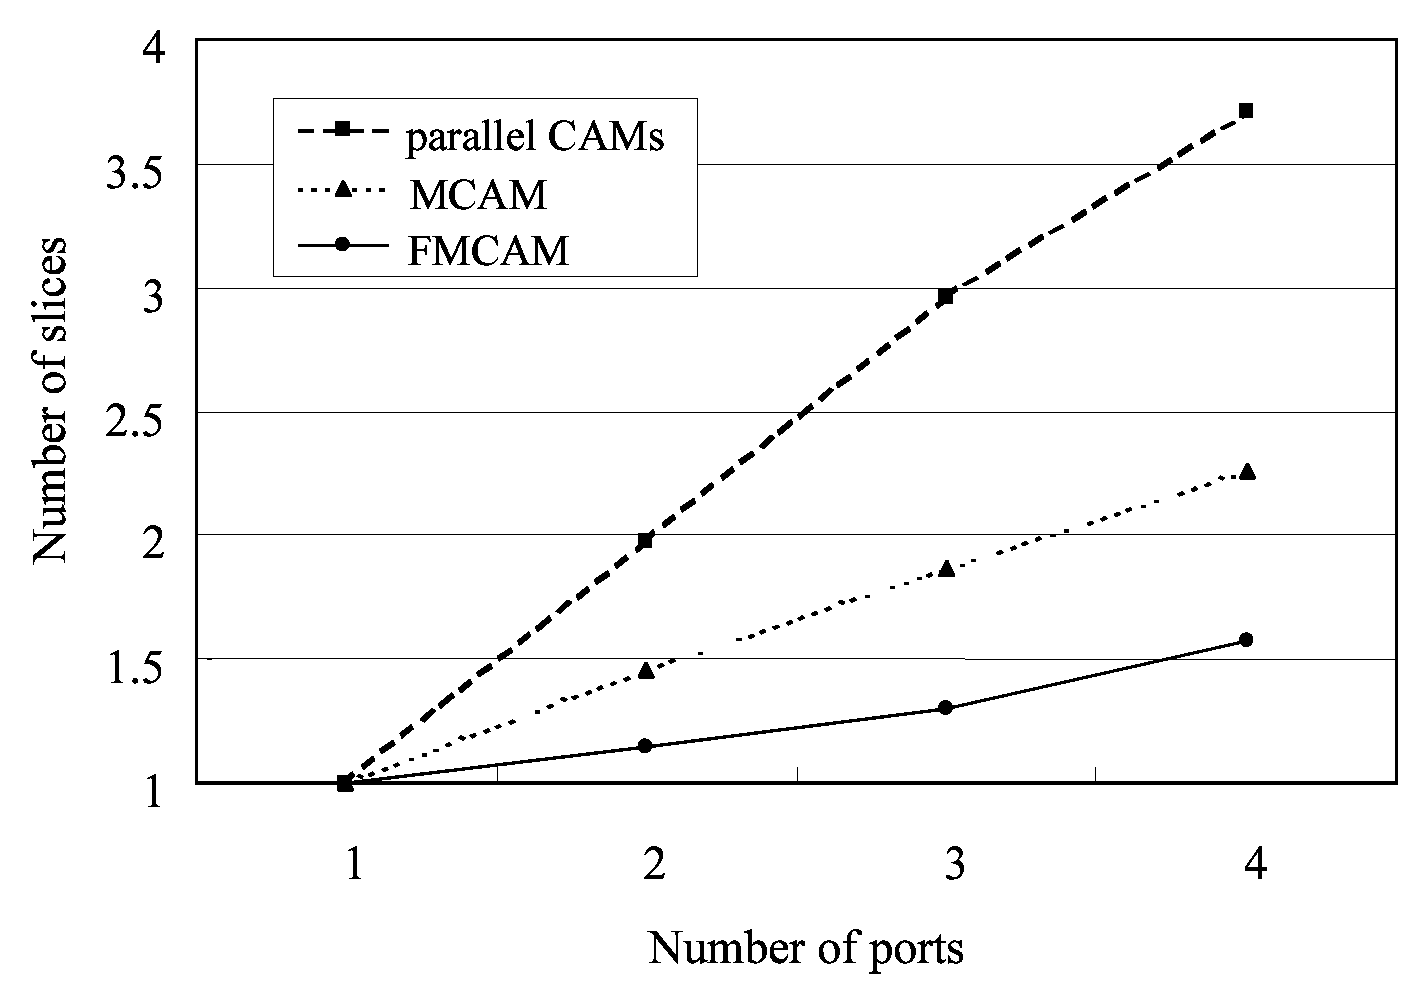
\includegraphics[width = 12cm,  height = 12 cm, keepaspectratio, clip]{./pics/para_gra.eps}
			\end{center}
			\caption{FMCAM,MCAM及び並列CAMのハードウェア量の比較.}
%			\ecaption{Device resources of FMCAM, MCAM and parallel CAMs.}
		\label{para_gra}
	\end{figure}%
%figure

\end{enumerate}

\clearpage

%/**********************************************************************/
%		Adapted FMCAMを解説する章
%/**********************************************************************/
\section{テーブルルックアップ用マルチポートCAM}
\label{lbl_cp4_adpt_fmcam}

マルチメディアデータ処理におけるボトルネックなっていたテーブルルックアップ処理は,
従来のアーキテクチャでは並列化が困難であることをこれまで述べた\cite{vcimiy00, fr50001}.
そこで,並列一致検索能力の高いFMCAMをテーブルルックアップ処理に利用することで
効果的な変換処理の実現が期待できる.

図 \ref{re_fmcam}に,マルチメディアデータ処理向けマルチポートCAM (Adapted FMCAM:Adapted Flexible Multi-ported 
Content Addressable Memory)の全体図を示す.
基本的な概観は,図 \ref{fmcam}と同様であるが,テーブルルックアップ処理にハミング距離を検索する必要は無いと判断し,
これに関するポートは除いてある.
図 \ref{re_fmcam_block}に,Adapted FMCAMのモジュール構成を示す.
図 \ref{fmcam_block}に示した,これまでのFMCAM (以下,Original FMCAMと呼ぶ)の構成と異なり,セレクタモジュールはポートモジュールに
組み込み,まとめてポートブロック (Port block)として設計の容易さを実現した.
また,カテゴリモジュールはリングカウンタと共に1つのコントローラとし,
図 \ref{memory_space}に示すように,Adapted FMCAMの制御及びデータの入出力を1つのメモリ空間にまとめた.
これによって,データの入出力,制御が全てアドレスを設定することで可能となり,初期データの入力等のピンを不要とし,
Adapted FMCAMの制御を一元化することが可能となった.
更に,これまでのコンテンツモジュールからリングカウンタ等を除いてカテゴリブロック (Category block)とした.
カテゴリブロックは,1ポートのSRAMを用いて多バンク構造としたため,LSI実装時に
スタンダードメモリセルを使用できるようになった.

この節では以降,\ref{lbl_cp4_fmcam}節で述べた,FMCAMをマルチメディアデータ処理に
活用するために施した3つの工夫について述べる.

% figure*
	\begin{figure}[tbh]
	\centering
		\begin{center}
			\includegraphics[width = 12cm, height = 12cm, keepaspectratio, clip]{./pics/re_fmcam.eps}
%		\caption{Input/Output configuration overview of the FMCAM architecture.}
		\caption{Adapted FMCAMの全体図.}
		\label{re_fmcam}
		\end{center}
	\end{figure}%
%\vspace{-3mm}
% figure*

% figure*
	\begin{figure}[tbh]
	\centering
		\begin{center}
			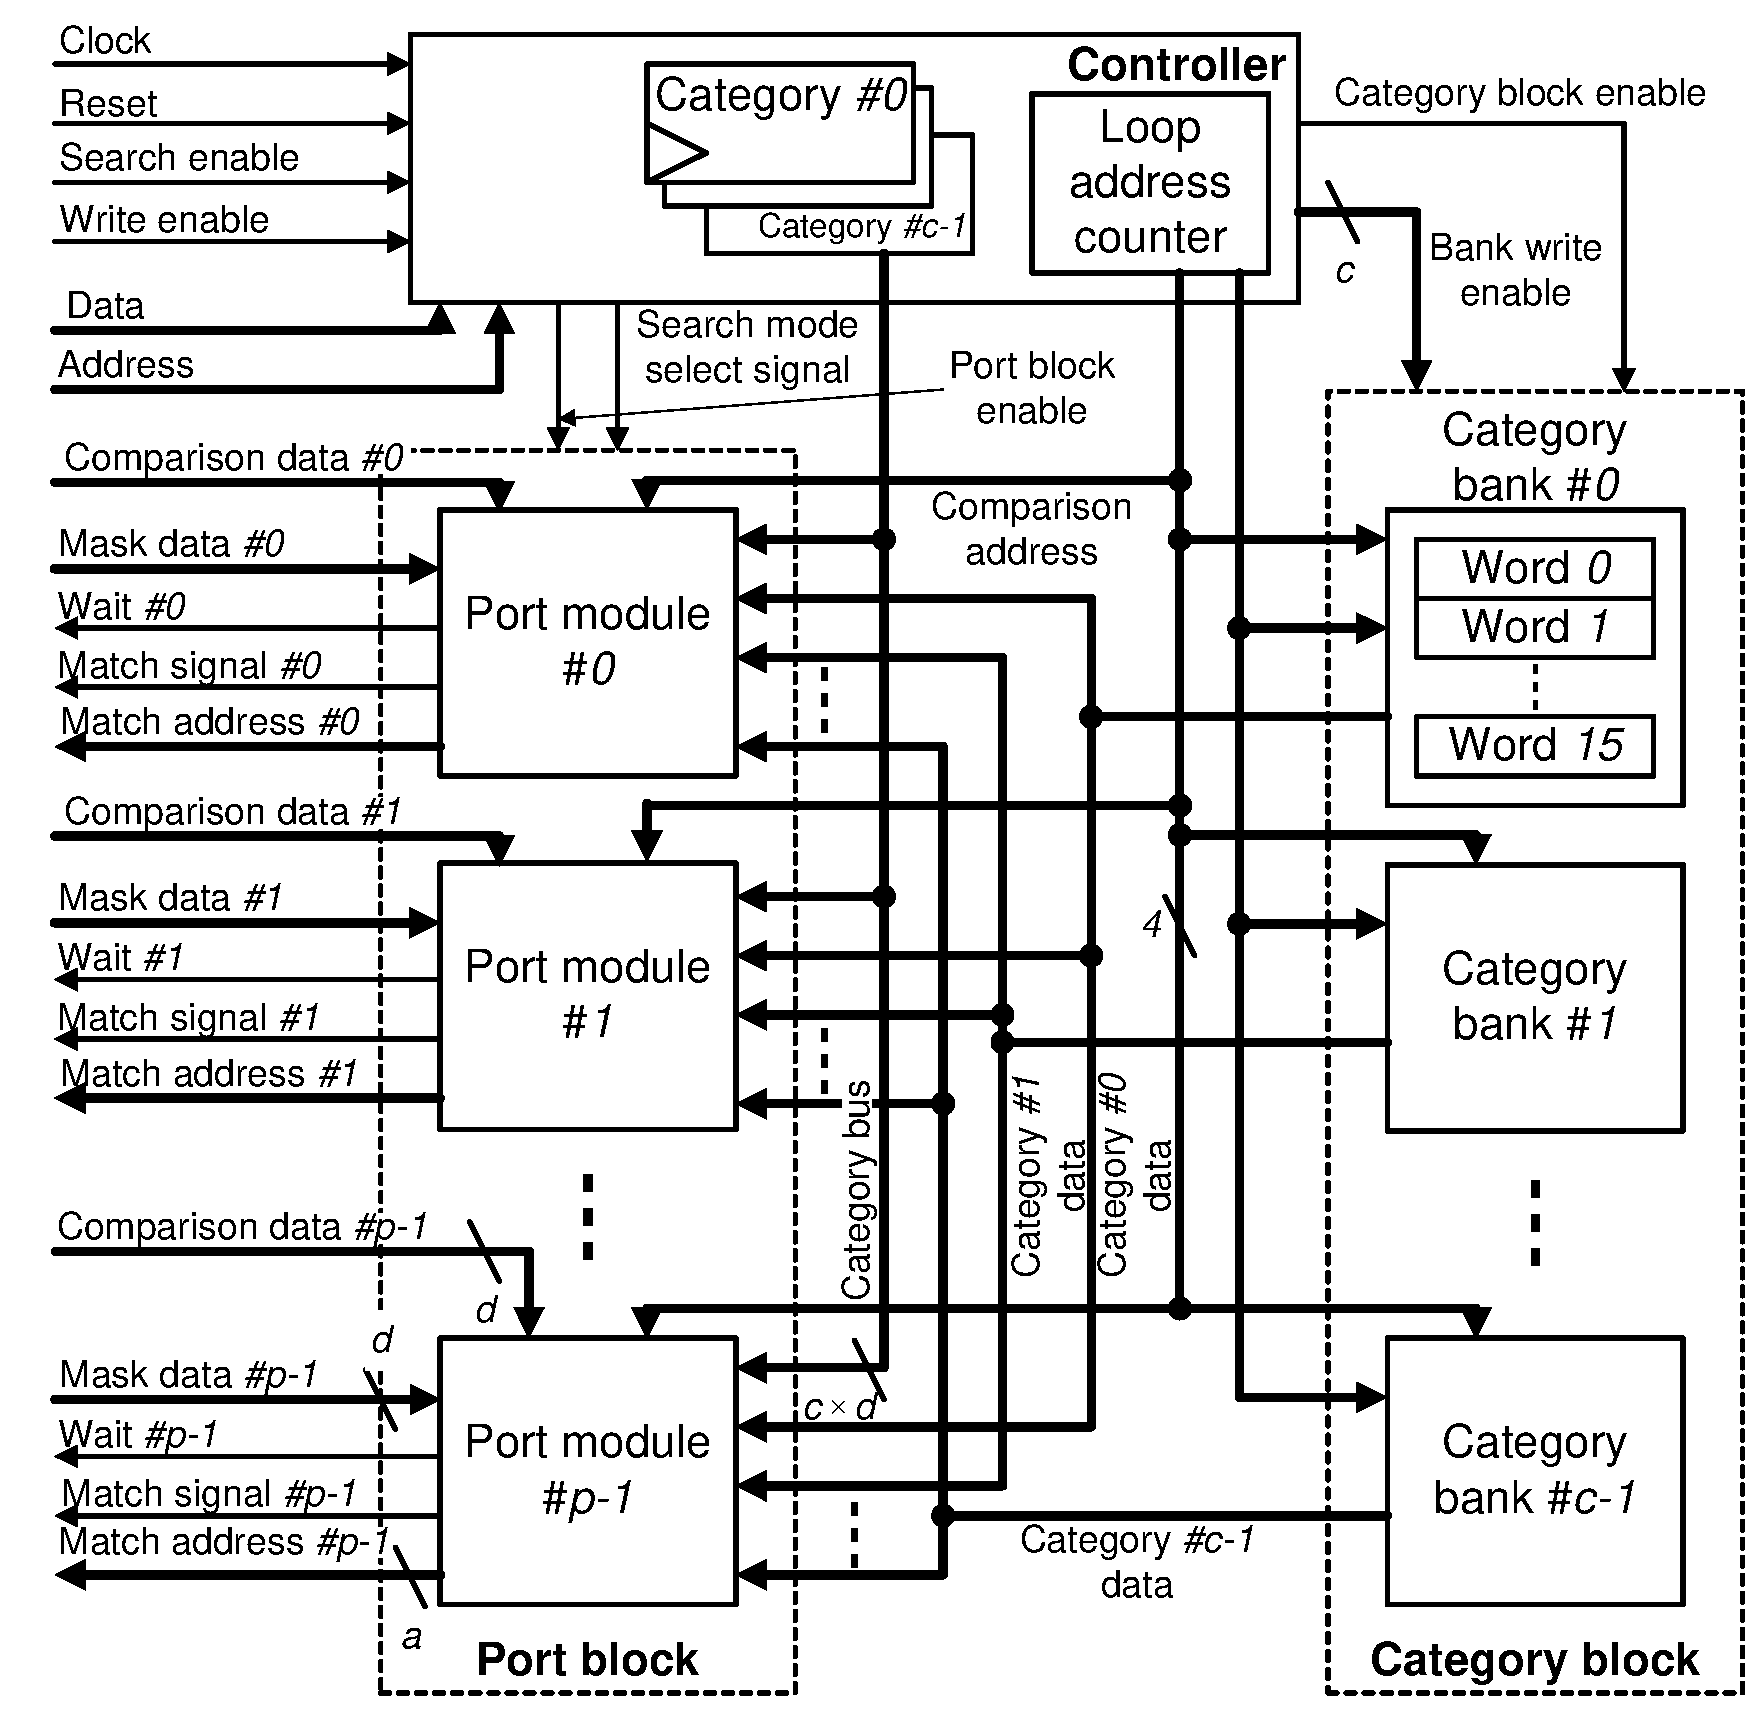
\includegraphics[width = 14cm, height = 14cm, keepaspectratio, clip]{./pics/re_fmcam_block.eps}
%		\caption{Detailed block diagram of the adapted FMCAM.}
		\caption{Adapted FMCAMのブロック図.}
		\label{re_fmcam_block}
		\end{center}
	\end{figure}%
%\vspace{-3mm}
% figure*

% figure*
	\begin{figure}[bht]
	\centering
		\begin{center}
			\includegraphics[width = 7cm, height = 7cm, keepaspectratio, clip]{./pics/memory_space.eps}
%		\caption{Hardware configuration.}
		\caption{Adapted FMCAMのメモリ空間.}
		\label{memory_space}
		\end{center}
	\end{figure}%
%\vspace{-3mm}
% figure*


\subsection{マルチプル/シングルサーチモード (Multiple/Single Search Mode)}
\label{lbl_cp4_adpt_fmcam_mulsin}
Original FMCAMは,マルチポート化に伴う比較器の増加を押さえるために,一般のCAMで用いられている
BPWP方式の変わりにBPBP方式を採用している.
これにより,\ref{lbl_cp4_fmcam_hyouka}節で示すように,AT積において優れた値を示すことができている.
しかしながら,リアルタイムに大容量のデータが配信される近年のマルチメディアアプリケーションを
高速に処理することを考慮すると,比較にかかるクロックサイクル数を更に削減し,BPWPの
処理クロックサイクル数に近づける必要がある.
ここで,一般にマルチメディアデータ処理におけるテーブルルックアップ処理の特徴を検討すると,符号化前のデータと,符号化後のデータは
必ず1対1であることが分かる.そのため一回の検索処理サイクルで,符号化前のデータに対する一致検索結果が出力された後は,
その以降のデータを調べる必要がない.
以上のことから,Adapted FMCAMは,
一致検索処理に2種類のモード,``マルチプルサーチモード (Multiple 
search mode)"と``シングルサーチモード (Single search mode)"を用意した.
これらのモードはコントローラからポートブロックを制御することで実現される.

図 \ref{slct_md_wv}に一致検索時の両モードの動作波形を示す.
図 \ref{slct_md_wv}-(a)の例は,マルチプルサーチモード,すなわちOriginal FMCAMの検索動作である.
このモードは比較対象データ内に,検索データと同一のものが複数存在している状況を前提としているため,
図中では1回のサーチタイム (Search time)で,2つのマッチシグナル (Match signal)が出力されている.
このサーチタイムにかかるクロックサイクル数は,アプリケーションによらず一定である.
図 \ref{slct_md_wv}-(b)の例は,Adapted FMCAMに,新たに追加された検索動作であるシングルサーチモードの動作波形である.
テーブルルックアップ処理は,1度マッチシグナルが出力された後は,検索処理をする必要がない.
そのため図中で示しているように,マッチシグナルが出力された後は,
直ちに次の検索動作へ移行することを可能とした.
結果として1回のサーチタイムが短くなり,次々と新しいデータの検索処理を行うことが可能となった.


\subsection{カウンタ値設定モード (Counting Value Setting Mode)}
\label{lbl_cp4_adpt_fmcam_cnt}

Adapted FMCAMは,比較器の削減のためにBPBPの採用だけでなく,
\ref{cat_syori}節で述べた,カテゴリ分け処理も採用している.
この工夫を行うことで,各ポートとも,全てのデータを検索する必要が無く,
1つのカテゴリバンクに検索範囲を制限することが可能となった.
しかしながら,1つのカテゴリバンクに格納できるワード数は固定される.
そのため,このワード数がそのままループアドレスカウンタの最大値となり,一致検索処理に
必要とするクロックサイクル数となっていた.
一般に1つのカテゴリに格納するデータの個数はアプリケーションによって異なり,
検索処理に無効なワードも保存しなければならない場合が生じる.
図 \ref{addr_stg_wv}-(a)の例に示すように,カテゴリバンクに4つの無効なデータが存在している場合,
検索データが入力されたとしても,始めの4クロックサイクルは,検索処理に関係がないため,
直接処理時間の増加につながることとなる.
この問題を解決するために,Adapted FMCAMは,ループアドレスカウンタによる検索クロックサイクル数を,
ユーザが任意に変更できる仕様にした.
図\ref{addr_stg_wv}-(b)の例に示すように,本来であれば1回の検索処理に16クロックサイクルかかるところを,
12クロックサイクルでループするように設定することが可能である.この例の場合は,図 \ref{addr_stg_wv}-(a)
と比較して,サーチタイムが約2分の1となっていることが分かる.



\subsection{カテゴリ結合モード (Scalability of Categorization Structure)}
\label{lbl_cp4_adpt_fmcam_stcat}

カテゴリ分け処理を行っているCAM \cite{mot12m, scharc}の多くは,1カテゴリの容量を変化させることはできない.
そのため,1つのカテゴリに格納するためのデータ数が許容量を超えるアプリケーションには,適用が難しくなる.
そこで,Adapted FMCAMは,広範囲のアプリケーションに適用できるように,カテゴリバンクの格納
にスケーラビリティを持たせるように工夫した.
すなわち,あるカテゴリのデータ群が1つのカテゴリ容量に格納できない場合には,2つのカテゴリを結合して
1つのカテゴリとすることを可能とした.
これによって適用できるアプリケーションの幅が広がることが期待できる.
一致検索処理に必要なクロックサイクル数は倍となるが,
シングルサーチモードを適用した場合にはクロックサイクル数を削減することが可能である.

% figure*
	\begin{figure}[tbh]
	\centering
		\begin{center}
			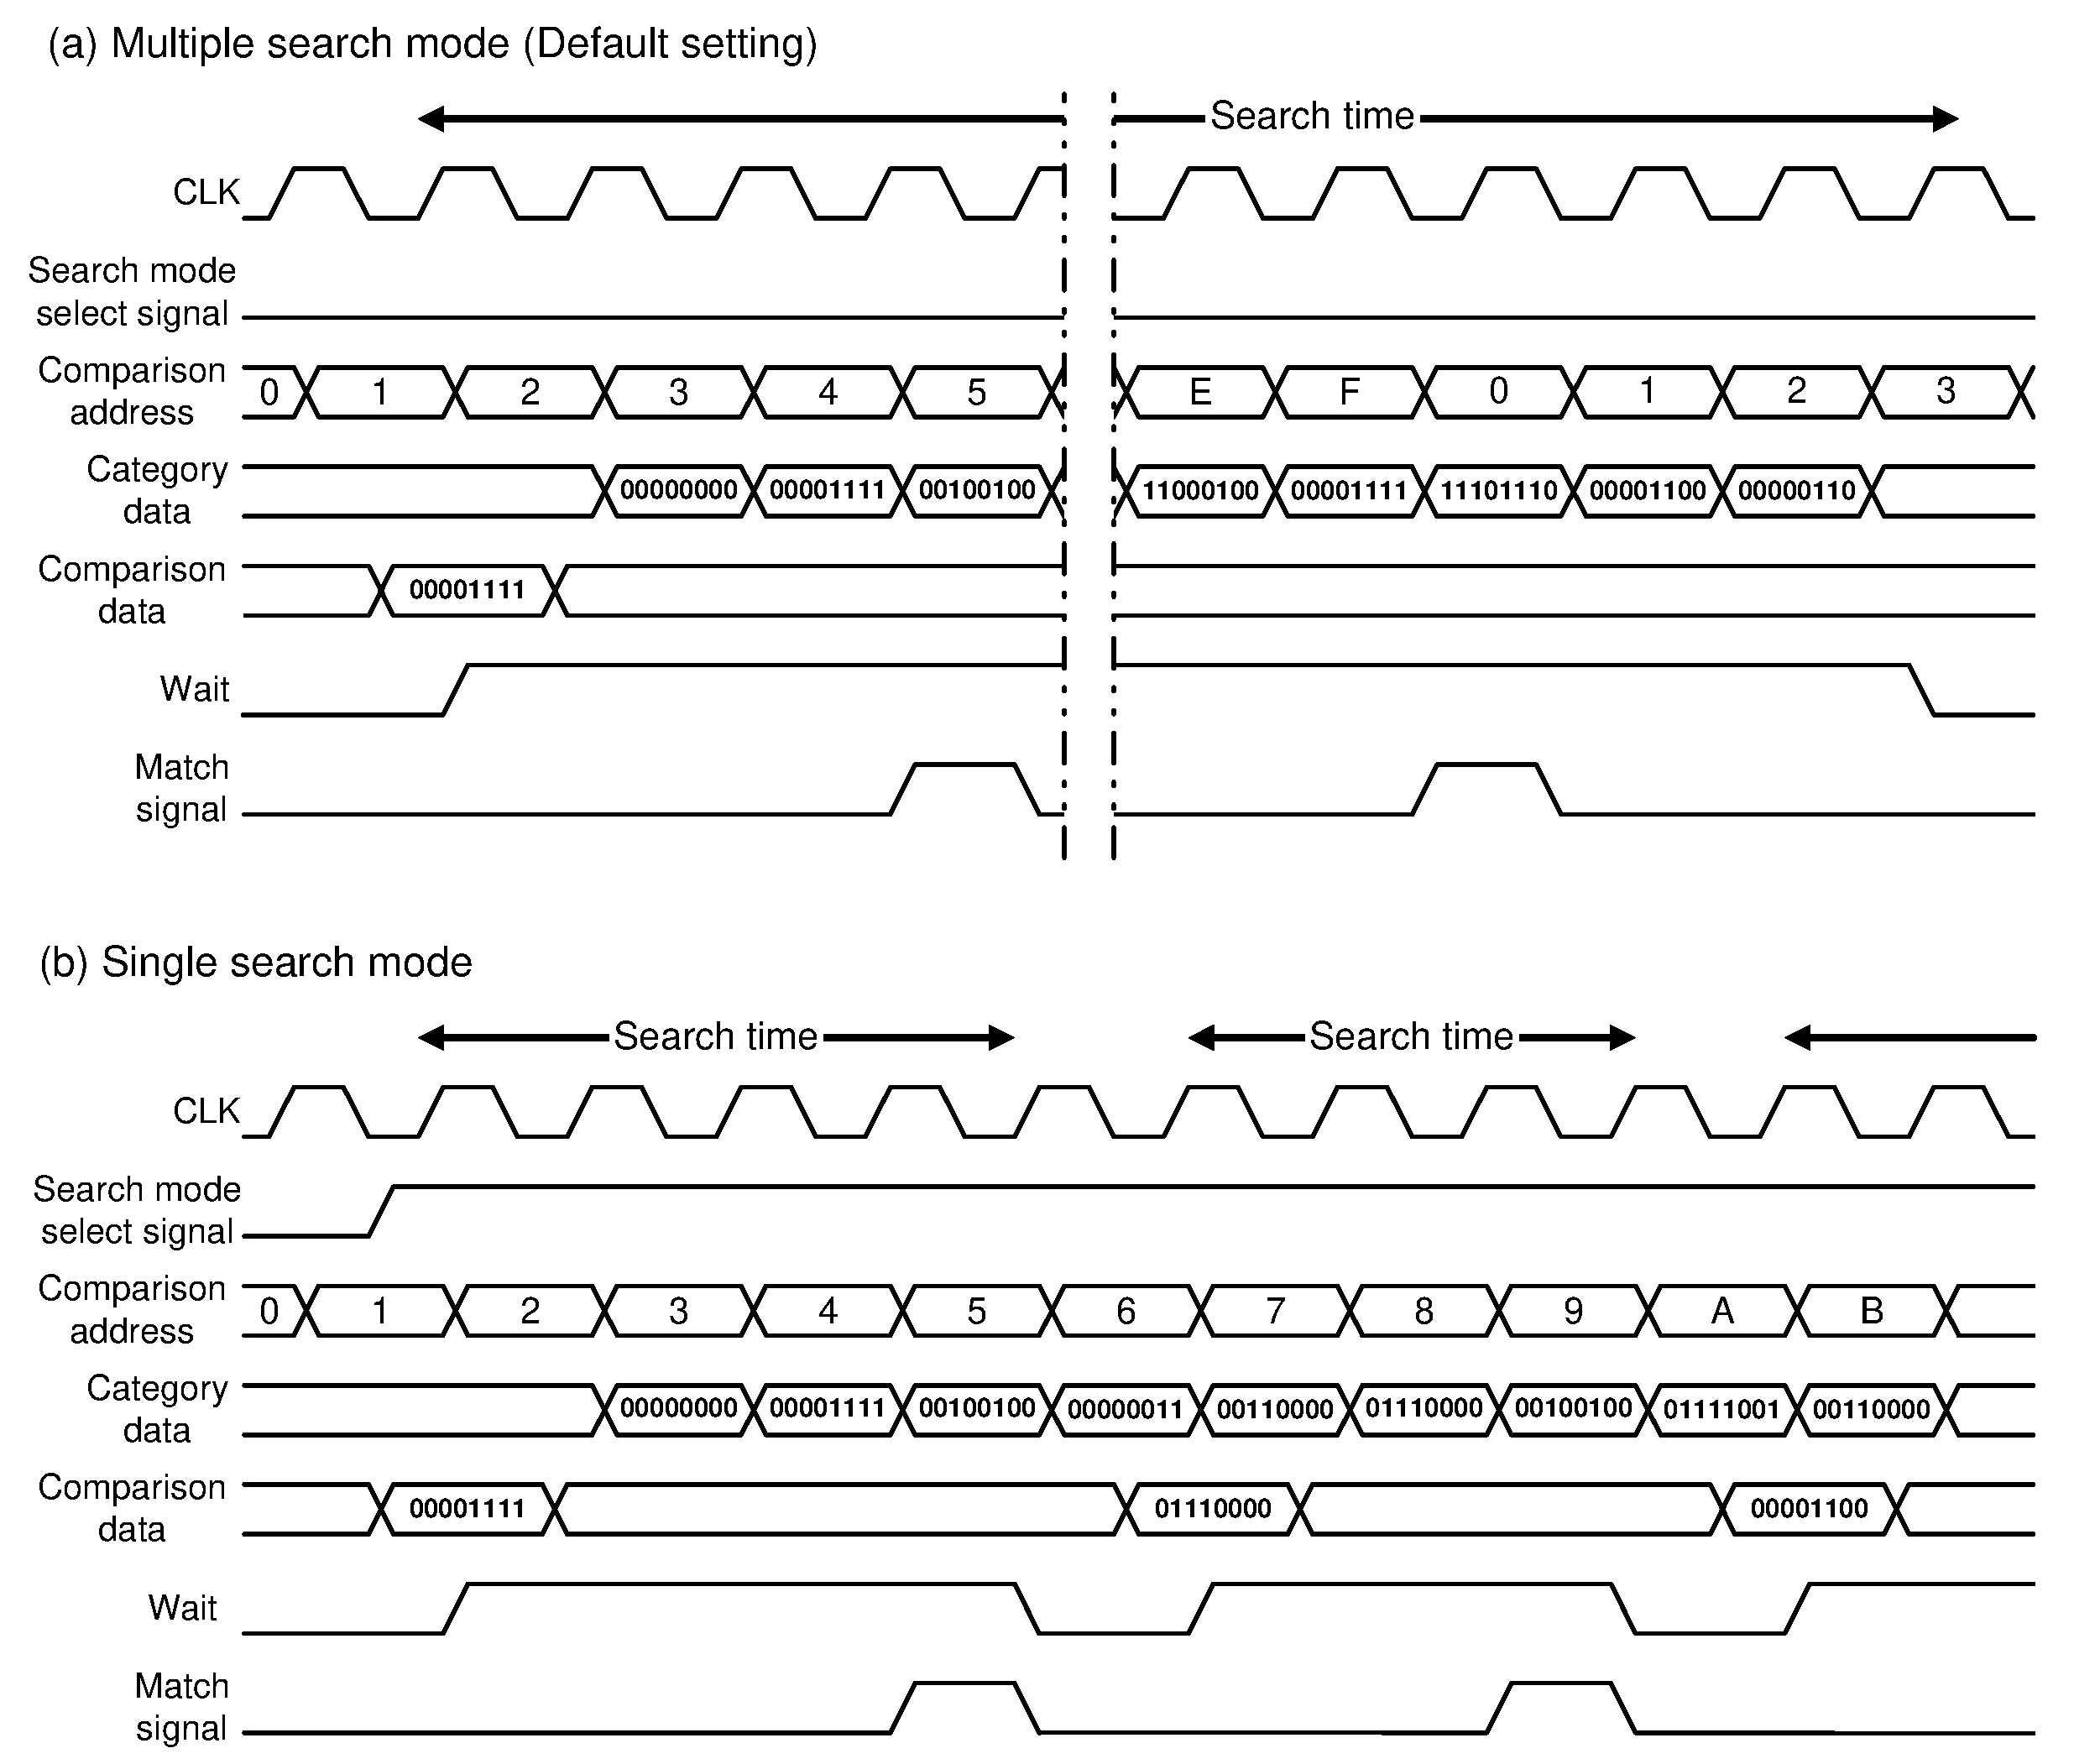
\includegraphics[width = 14cm, height = 14cm, keepaspectratio, clip]{./pics/slct_md_wv.eps}
%		\caption{Two search waveforms of the adapted FMCAM: (a) Multiple search mode, 
%						applied if multiple matches may exist, (b) Single search mode, 
%						applied if the search problem has a single well defined match.}
		\caption{Adapted FMCAMによる一致検索時の動作波形:
					(a) マルチプルサーチモード,(b) シングルサーチモード.}
		\label{slct_md_wv}
		\end{center}
	\end{figure}%
%\vspace{-3mm}
% figure*

% figure*
	\begin{figure}[tbh]
	\centering
		\begin{center}
			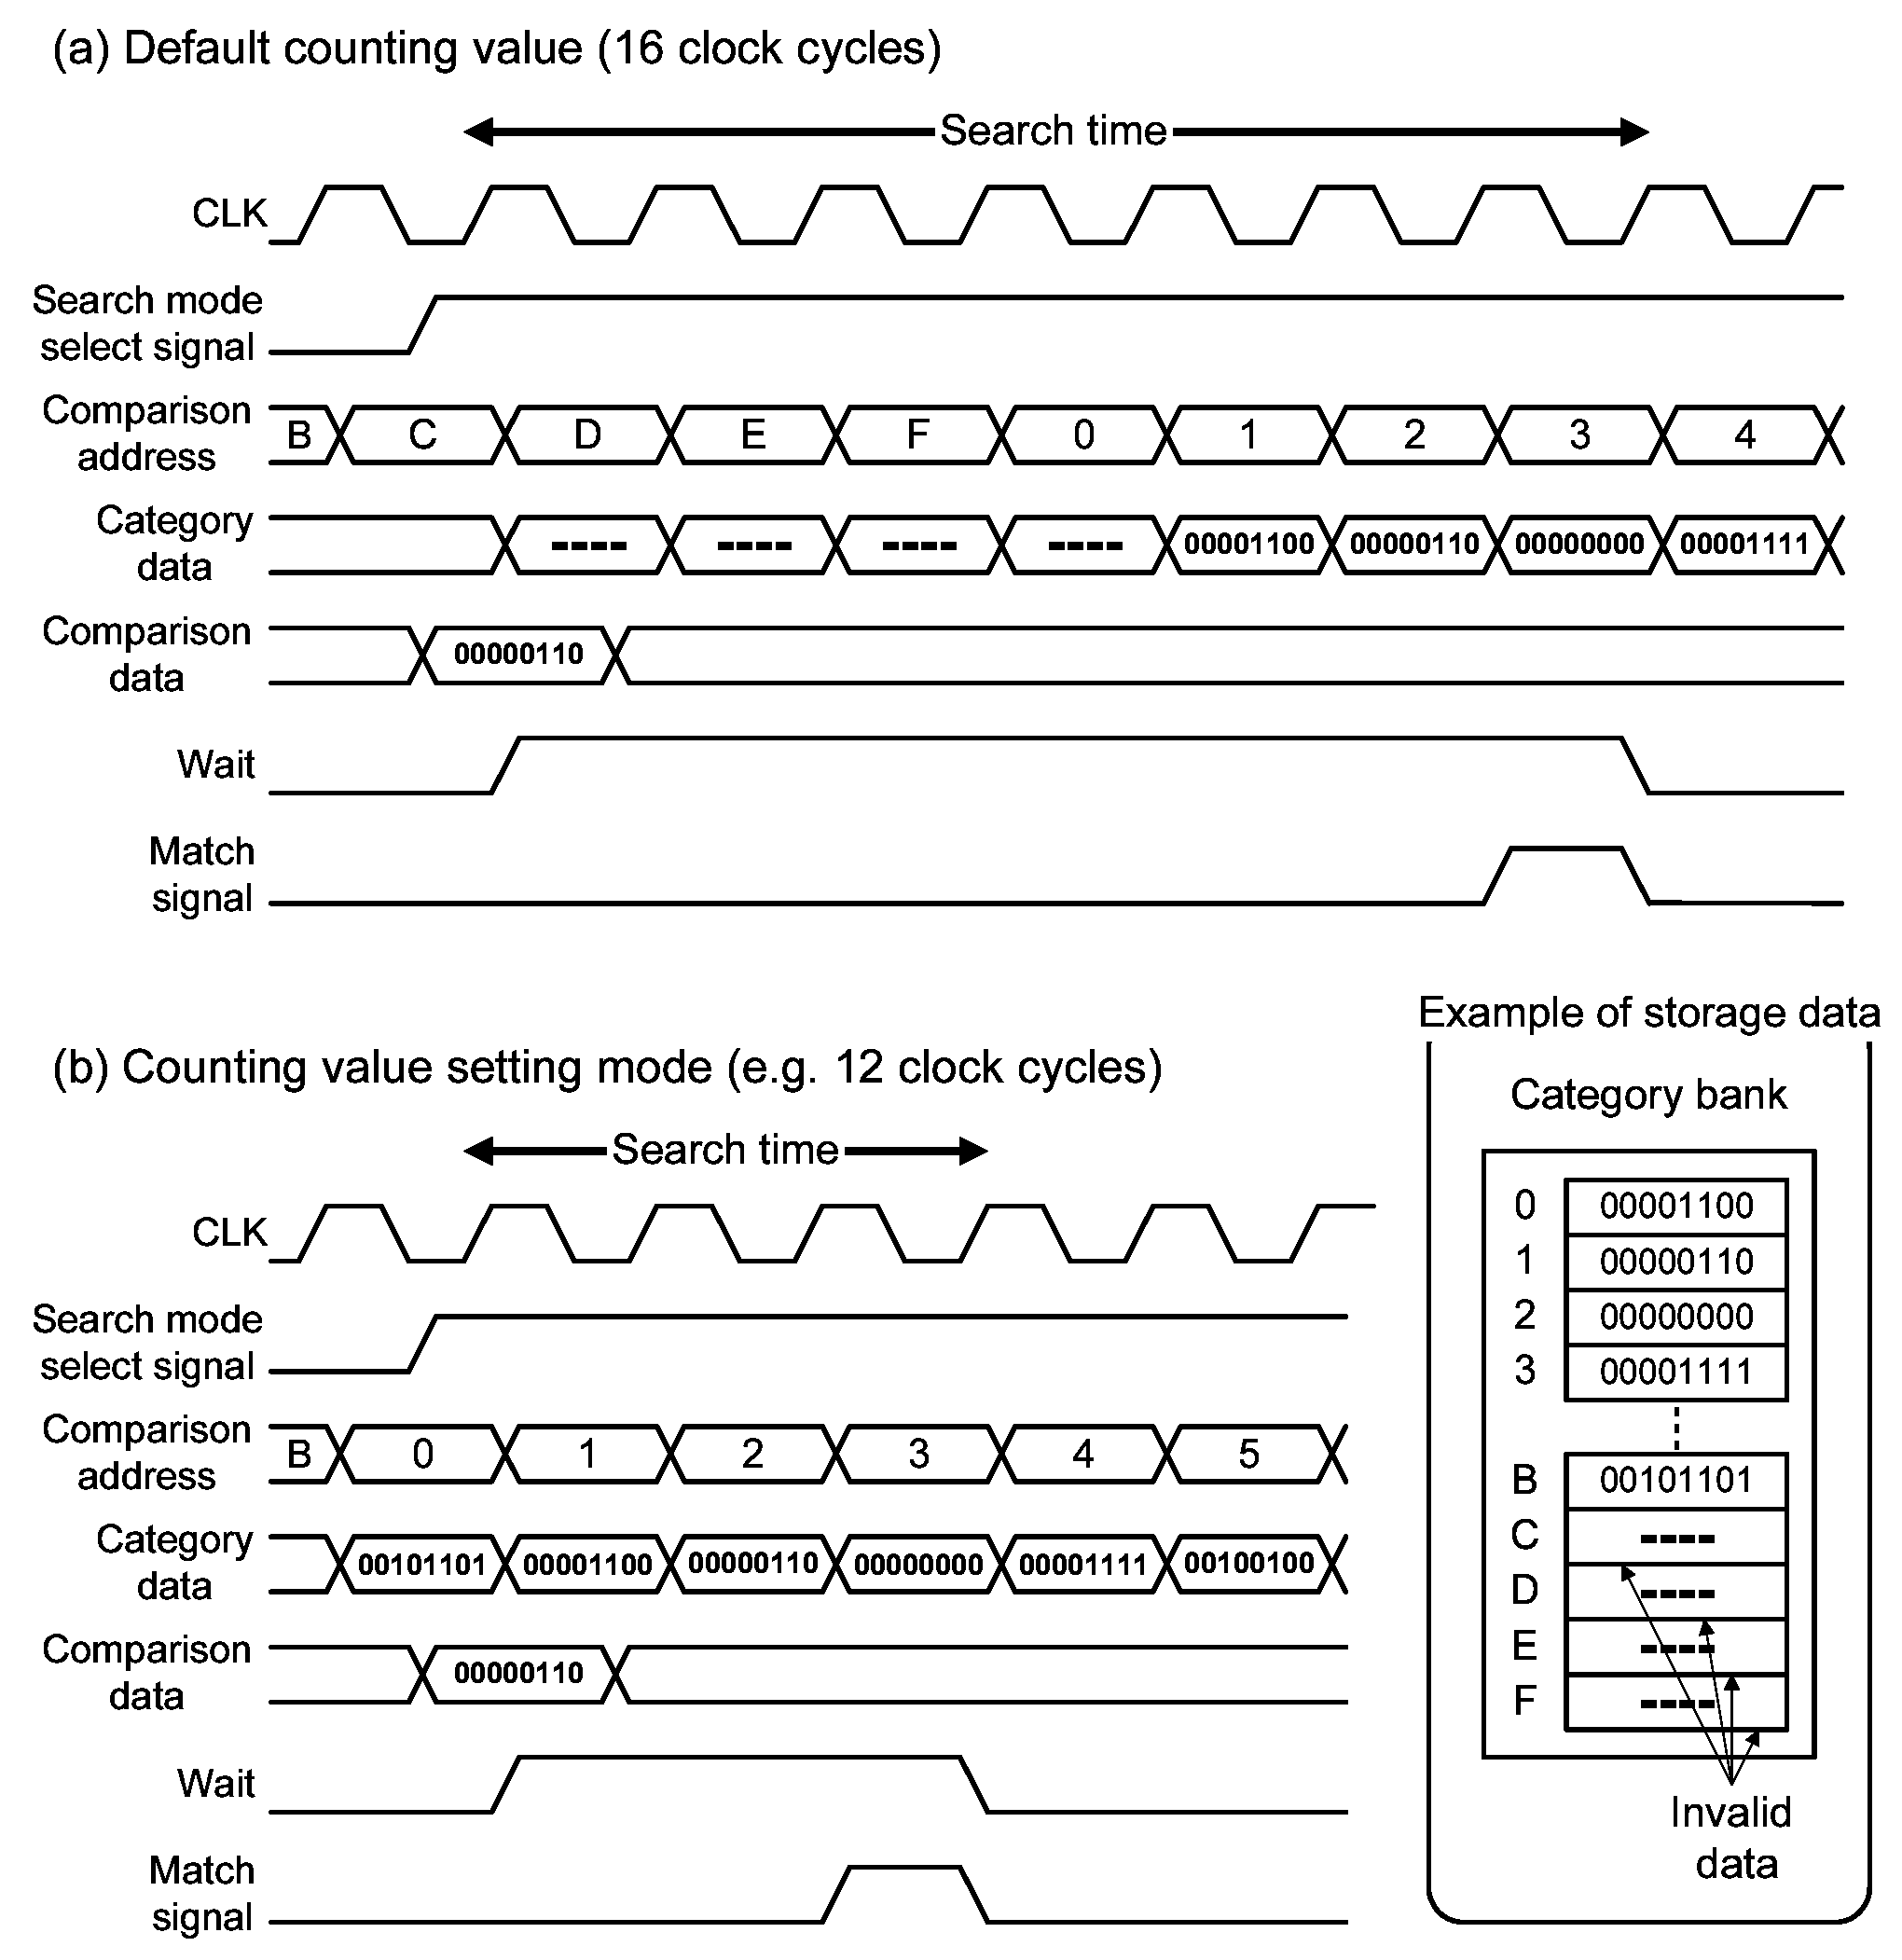
\includegraphics[width = 14cm, height = 14cm, keepaspectratio, clip]{./pics/addr_stg_wv.eps}
%		\caption{Two address counting waveforms of the adapted FMCAM: (a) Default counting mode, 
%						(b) Counting value setting mode.}
		\caption{Adapted FMCAMによる一致検索時のカウンタ動作:
					(a) 通常モード,(b) カウンタ値設定モード.}
		\label{addr_stg_wv}
		\end{center}
	\end{figure}%
%\vspace{-3mm}
% figure*

\clearpage

\section{アーキテクチャ}
\label{lbl_cp4_adpt_fmcam_arch}
Adapted FMCAMは,大きく分けてポートブロック (Port block),カテゴリブロック (Category block),
及びコントローラ (Controller)から構成される.これらは,互いに機能を独立させて設計されているため,
ポート数の増減はポートモジュールの個数を変化させるだけでよく,スケーラビリティ性が高い.
以下の節では,各ブロックの動作概要及び構成を述べる.

\subsection{ポートブロック (Port block)}
\label{lbl_cp4_adpt_fmcam_prtblk}
図 \ref{re_fmcam_block}に示すように,ポートブロックは$p$個のポートモジュールから構成される.
このモジュールの個数がAdapted FMCAMのポート数及び並列処理能力に反映されるため,
ポートモジュールの個数が多いほど検索能力が向上する.
図 \ref{port_module}に,ポートモジュールの構成を示す.
このモジュールは,$d$-bitの検索データ及びマスクデータを入力することができ,
1 bitの検索結果信号と,そのデータが格納されている$a$-bitのアドレスを出力することができる.
一致検索処理に関して,ポートモジュールは他のポートモジュールと同期を取ることなく動作させることができるため,
検索データを入力させたならば,直ちに検索処理に取り掛かることが可能である.

%figure*
	\begin{figure}[tbh]
	\centering
		\begin{center}
			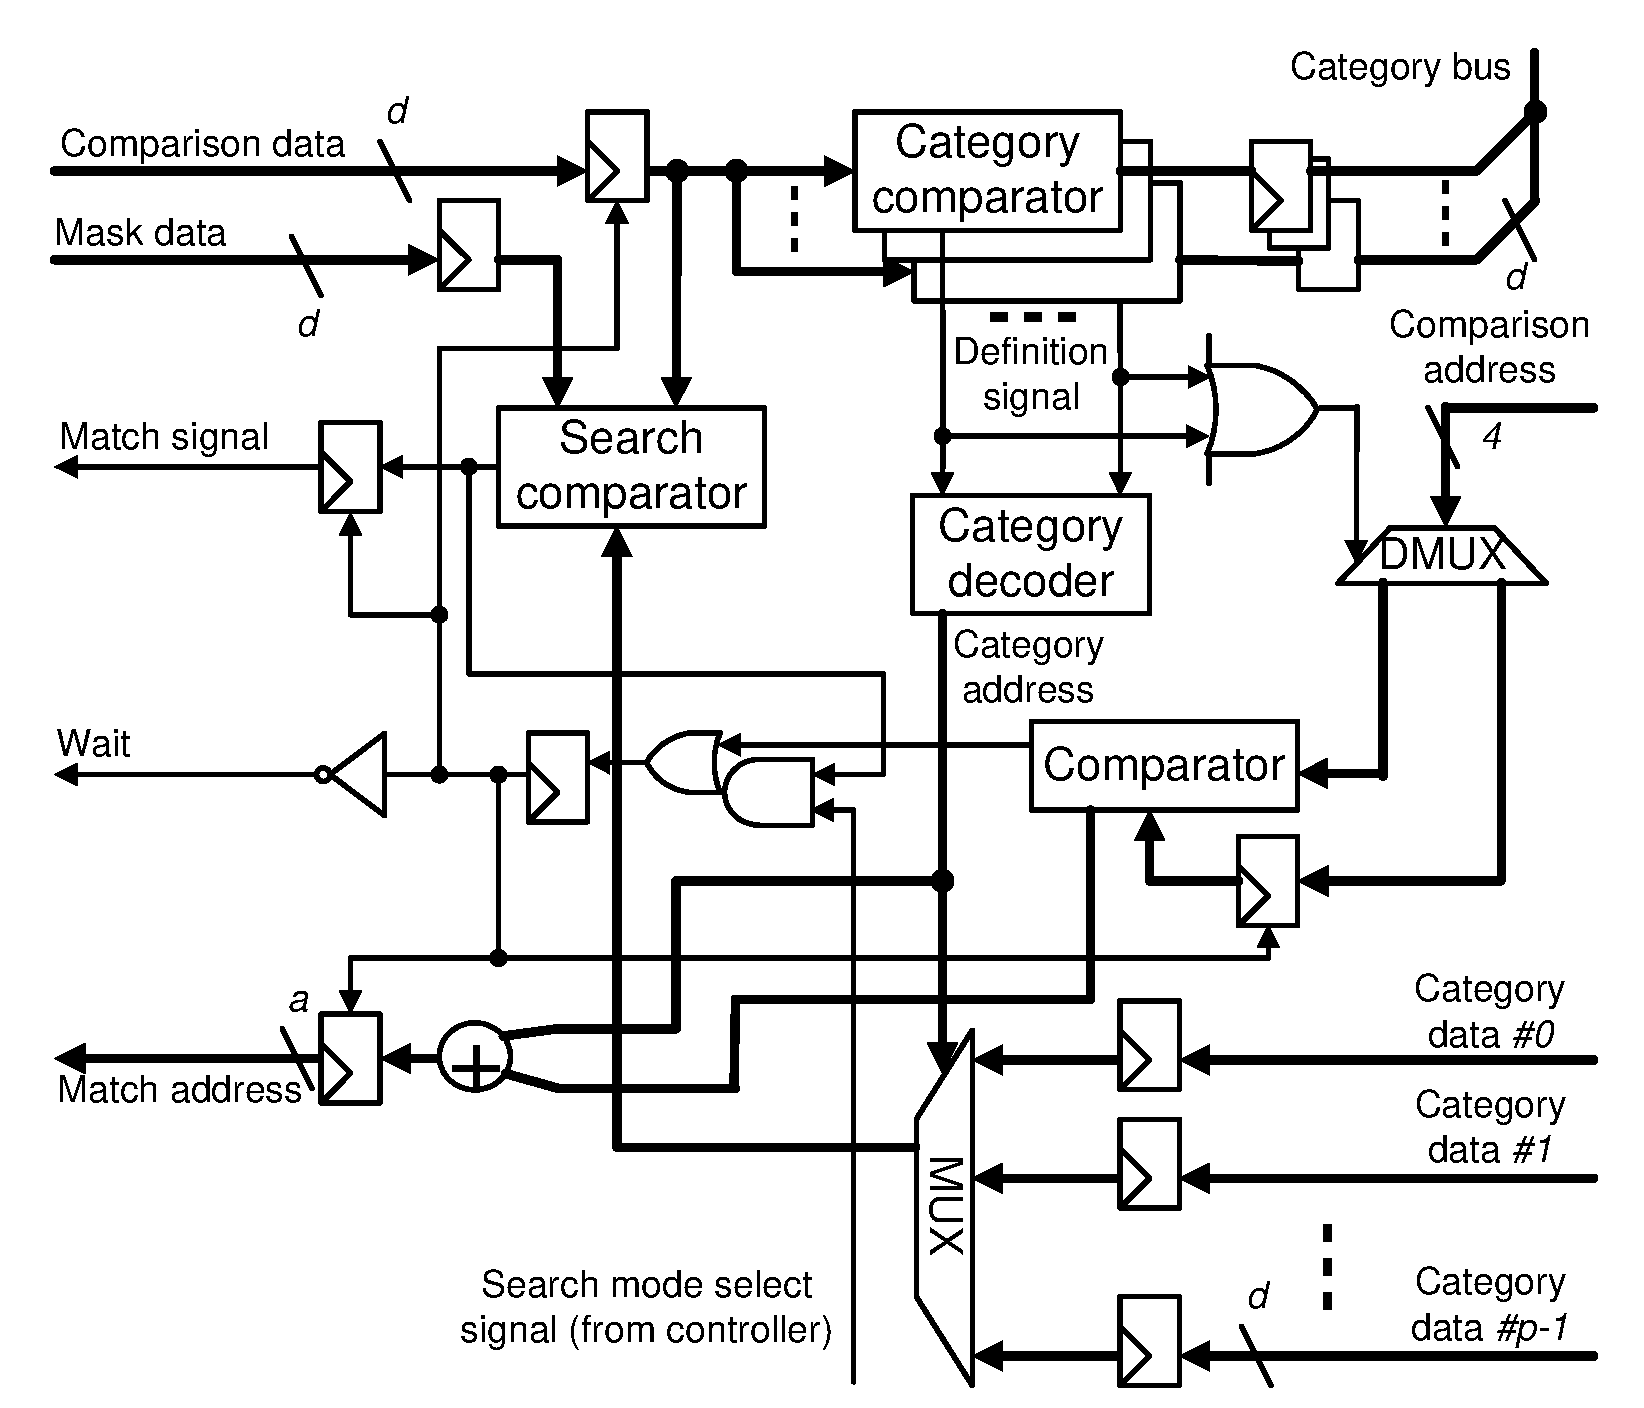
\includegraphics[width = 12cm, height = 12cm, keepaspectratio, clip]{./pics/port_module.eps}
%		\caption{Block diagram of a port module of the adapted FMCAM.}
		\caption{Adapted FMCAMにおけるポートモジュールのブロック図.}
		\label{port_module}
		\end{center}
	\end{figure}%
%\vspace{-3mm}
% figure*

Adapted FMCAMのポートモジュールは,大きく分けて以下に示す9種類のユニットと複数個のレジスタ及び論理回路から構成される.

\begin{itemize}
\item 一致検索用比較器 (Search comparator)  $\times$  $1$ 
\item カテゴリ選択用比較器 (Category comparator)  $\times$  $c-1$
\item ループアドレスカウンタ用比較器 (Comparator)  $\times$  $1$
\item カテゴリデコーダ (Category decoder)  $\times$  1
\item マルチプレクサ (MUX: MUltipleXer) $\times$  1
\item デマルチプレクサ (DMUX: DeMUltipleXer) $\times$  1
\end{itemize}

ポートモジュールに検索データが入力されたならば,カテゴリ選択用比較器は,データ内のカテゴリを決定する
ビット箇所とコントローラ内のカテゴリデータを比較し,カテゴリ選択信号 (Definition signal)を出力する.
この信号はカテゴリデコーダにてカテゴリアドレスに変換され,マルチプレクサを制御する.
マルチプレクサは,検索データに属しているカテゴリのデータを選択し,これらのデータは順次
一致検索用比較器に送られる.一致検索用比較器は送られてきたカテゴリのデータと検索データを比較し,
一致したものがあれば一致信号を及びそのアドレスを出力する.上記の処理と並行してループアドレスカウンタから送られてくる
アドレスは,カテゴリ選択信号が出力された際にレジスタに格納される.
ここで格納されたレジスタはループアドレスカウンタが再び同じアドレスを送信するまで保持されることとなる.
この間が1回の一致検索処理にかかる時間となる.また,ループアドレスカウンタは全ての
ポートモジュールにブロードキャストされているが,格納するレジスタは各ポートモジュール固有なため,
各ポート一致検索に同期を取る必要が無い.
以上は,マルチプルサーチモードの検索行程となるが,シングルサーチモードが選択されている場合,
そのイネーブル信号 (Search mode select signal)が,コントローラから入力され,
一致検索結果とAND演算された後に,直ちに各レジスタはリセットされることとなる.



\subsection{カテゴリブロック (Category block)}
\label{lbl_cp4_adpt_fmcam_catblk}

Adapted FMCAMは,比較器の配置を工夫することで,実装に関し様々な利点を
有している.
従来のCAMは,検索データと全比較対象データを並列に検索するため,メモリセル内に
比較のためのトランジスタを追加しなければならない.しかしながら,この手法は以下に示す
2つの問題がある.
\begin{enumerate}
\item CAMをLSIとして実装する際に,専用のCAMセルを設計,もしくは使用しなければならない.
そのため,動作速度及び面積において最適にカスタマイズされた,多くのスタンダードSRAMセルを使用することができない.
よって,実装面積も大きくなり,適用アプリケーションに制限が生じる.

\item マルチポート化が困難となる.通常のCAMセルをマルチポート化する場合ポート数分
XNORを構成するトランジスタを追加する必要が生じる.これは実装面積及び消費電力等の面で
問題がある.
\end{enumerate}

以上の問題を克服すべくいくつかの研究が行われているが\cite{schful, harcol},実現された例はない.
そこで,Adapted FMCAMは,比較器をメモリセルから分離し,ポートモジュールとしてまとめて配置することで,この問題を解決した.
ポートモジュール内の比較器には,各メモリセルからデータがブロードキャストされており,
検索データの入力にあわせて一致検索処理を行うことが可能である.
この方式を採用することによって,Adapted FMCAMはFPGA,ASICと実装ターゲットにとらわれることなく,
組み込みメモリやスタンダードメモリセルを使用することが可能となり,比較器全体の面積も削減している.
また,設計に要する時間も,通常のCAMと比較して短期間になることが期待され,実装面積も縮小されると考えられる.


\subsection{コントローラ (Controller)}
\label{lbl_cp4_adpt_fmcam_cntrl}
コントローラは,主としてカテゴリ情報を格納するレジスタとループアドレスカウンタによって構成される.
ユーザから格納されたカテゴリのデータはマスクによってビット位置を指定された後,各ポートモジュールに
ブロードキャストされる.ループアドレスカウンタは\ref{ring}節で述べたリングカウンタの動作と同一であり,アドレスを降順に
カウントし,最大値に達した後,0から再びカウントを開始する.
ただし,カウンタ値設定モードでカウンタの最大値が指定された場合は,その値でループを繰り返すことになる.


\section{FPGA/ASICへの実装結果}
\label{lbl_cp4_adpt_fmcam_impl}

Original FMCAMは,既存のCAMと比較してAT積で優れており,並列CAMと比較した場合にも
面積の増加度は低く抑えられていることを示した (表 \ref{atp_comb},\ref{para_gra}参照).この特徴はAdapted FMCAMにも備わっている.
この節では更に,FPGA及びASICへのAdapted FMCAMの実装結果をもとに,
動作周波数,及び面積のスケーラビリティ性について述べる.

Adapted FMCAMは,ハードウェア記述言語であるVerilog-HDLで設計した.
FPGAへの実装については,Xilinx社の開発ツールである,ISE Foundation 7.1iを
用い,論理合成はSynplicity社のSynplify Pro 8.1を使用した.ターゲットデバイスは,
Xilinx社のFPGAである,XC4VLX160を使用している.
これらの環境で,最大動作周波数と,換算ゲート数を算出した.
図 \ref{fpga_impl}に配置配線後のマッピング状況を示す.
ASICへの実装については,Synopsys社のDesign Compiler (バージョン2005.09)によって
90 nm CMOSテクノロジで論理合成を行った.
図 \ref{re_fmcam_asic}に,16ポートの合成結果を示す.

%figure
%		\vspace{3mm}
	\begin{figure}[tbh]
		\begin{center}
			\includegraphics[width = 14cm,  height = 14cm, keepaspectratio, clip]{./pics/fpga_impl.eps}
		\end{center}
		\caption{配置配線マッピング結果.}
%		\ecaption{Comparison process with a ring counter.}
		\label{fpga_impl}
	\end{figure}%	
%figure

% figure*
	\begin{figure}[t]
	\centering
		\begin{center}
			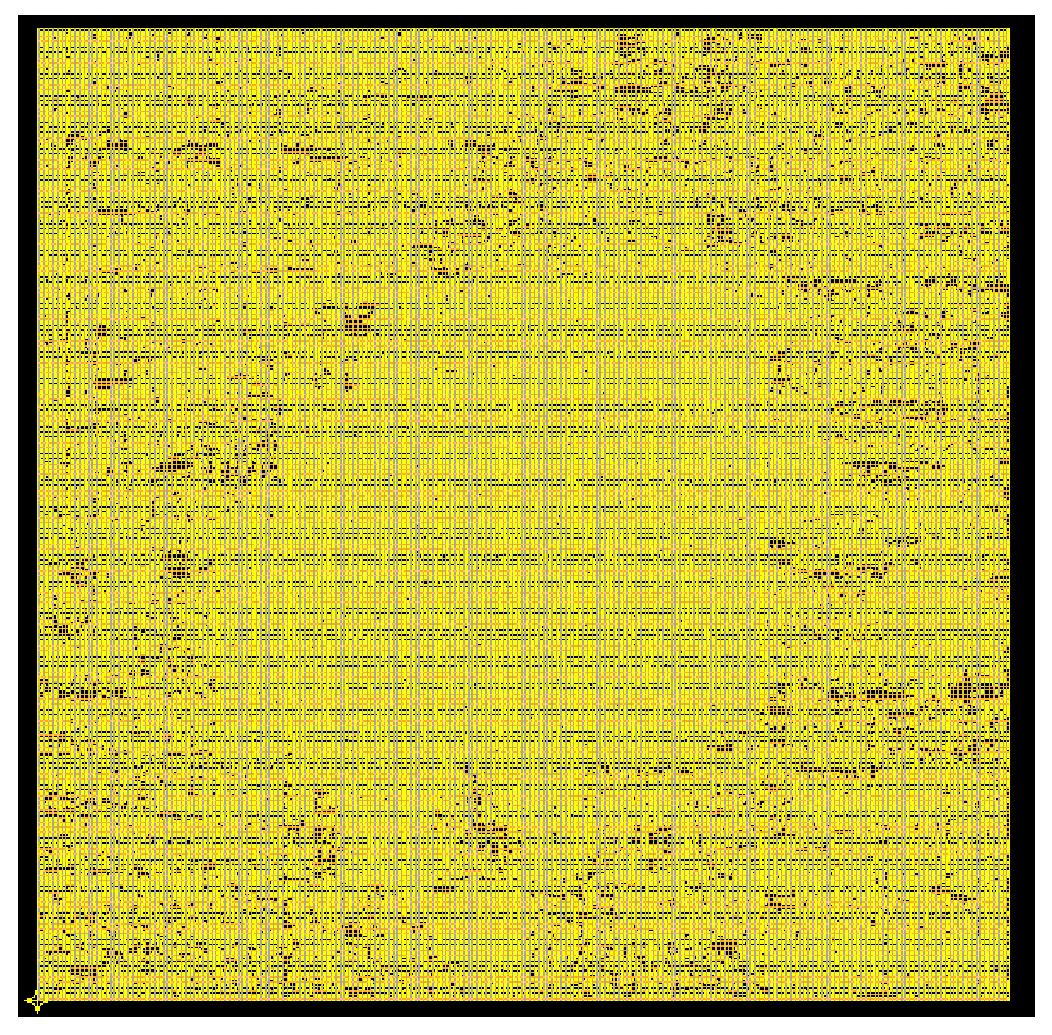
\includegraphics[width = 14cm, height = 14cm, keepaspectratio, clip]{./pics/re_fmcam_asic.eps}
%		\caption{FMCAM implementation results for the ASIC case ($90nm$ CMOS technology) as a function of the number of ports: 
%						(a) Maximum operating frequency, (b)Area consumption.}
		\caption{90 nm 7Cu CMOSテクノロジによる16ポートAdapted FMCAMの論理合成結果.}
		\label{re_fmcam_asic}
		\end{center}
	\end{figure}%
%\vspace{-3mm}
% figure*

以上の結果を元に,最大動作周波数
及び実装面積を見積もった.
Adapted FMCAMの各パラメータの緒元は,以下の通りである.

\begin{itemize}
\item アドレス値: $a = 8$
\item 1ワードのビット幅: $d = 32$
\item カテゴリ数: $c = 16$
\item ポート数: $p = 1 \sim 16$
\end{itemize}

図 \ref{impl_rslt_fpga}-(a)は,FPGAにおける論理合成後の最大動作周波数 (Synthesis maximum frequency),
及び配置配線後の最大動作周波数 (P\&R maximum frequency)を示している.
また,図 \ref{impl_rslt_asic}-(a)は,ASICにおける論理合成後の最大動作周波数を示している.
これらから分かるように,FPGA,ASICどちらに実装した場合にも.ポート数の増加と比較して,最大動作周波数の
低下は少ないことが分かる.特にASICの場合には,論理合成の結果ではあるが,
ポート数の増加に対し,最大動作周波数の制約条件である200 MHzに対し制約を満たさないことはなかった.
Adapted FMCAMは,ポート数の増加に対し,ポートモジュールを追加するだけで,コントローラ,及びコンテンツブロックには
影響を及ぼすことがない.ポートモジュールを増加するとポートブロックとコンテンツブロックをつなぐ信号線が
増加するため,FPGAにおける配置配線後の動作周波数は多少の減少が見られるが,大きいものではないと言える.
また,FPGAにおける配置配線後の動作周波数は,ポート数が8より大きい場合FPGAのリソースが不足したため,
破線で示す予測値となっている.
ASICへの実装に関しては,近年の多層配線技術の進歩により,90 nm CMOSテクノロジで7層程度まで使用できる.
よってポート数の増加に伴う信号線の増加に対しては,多層配線を効率よく利用することが重要となる.

% figure*
	\begin{figure}[t]
	\centering
		\begin{center}
			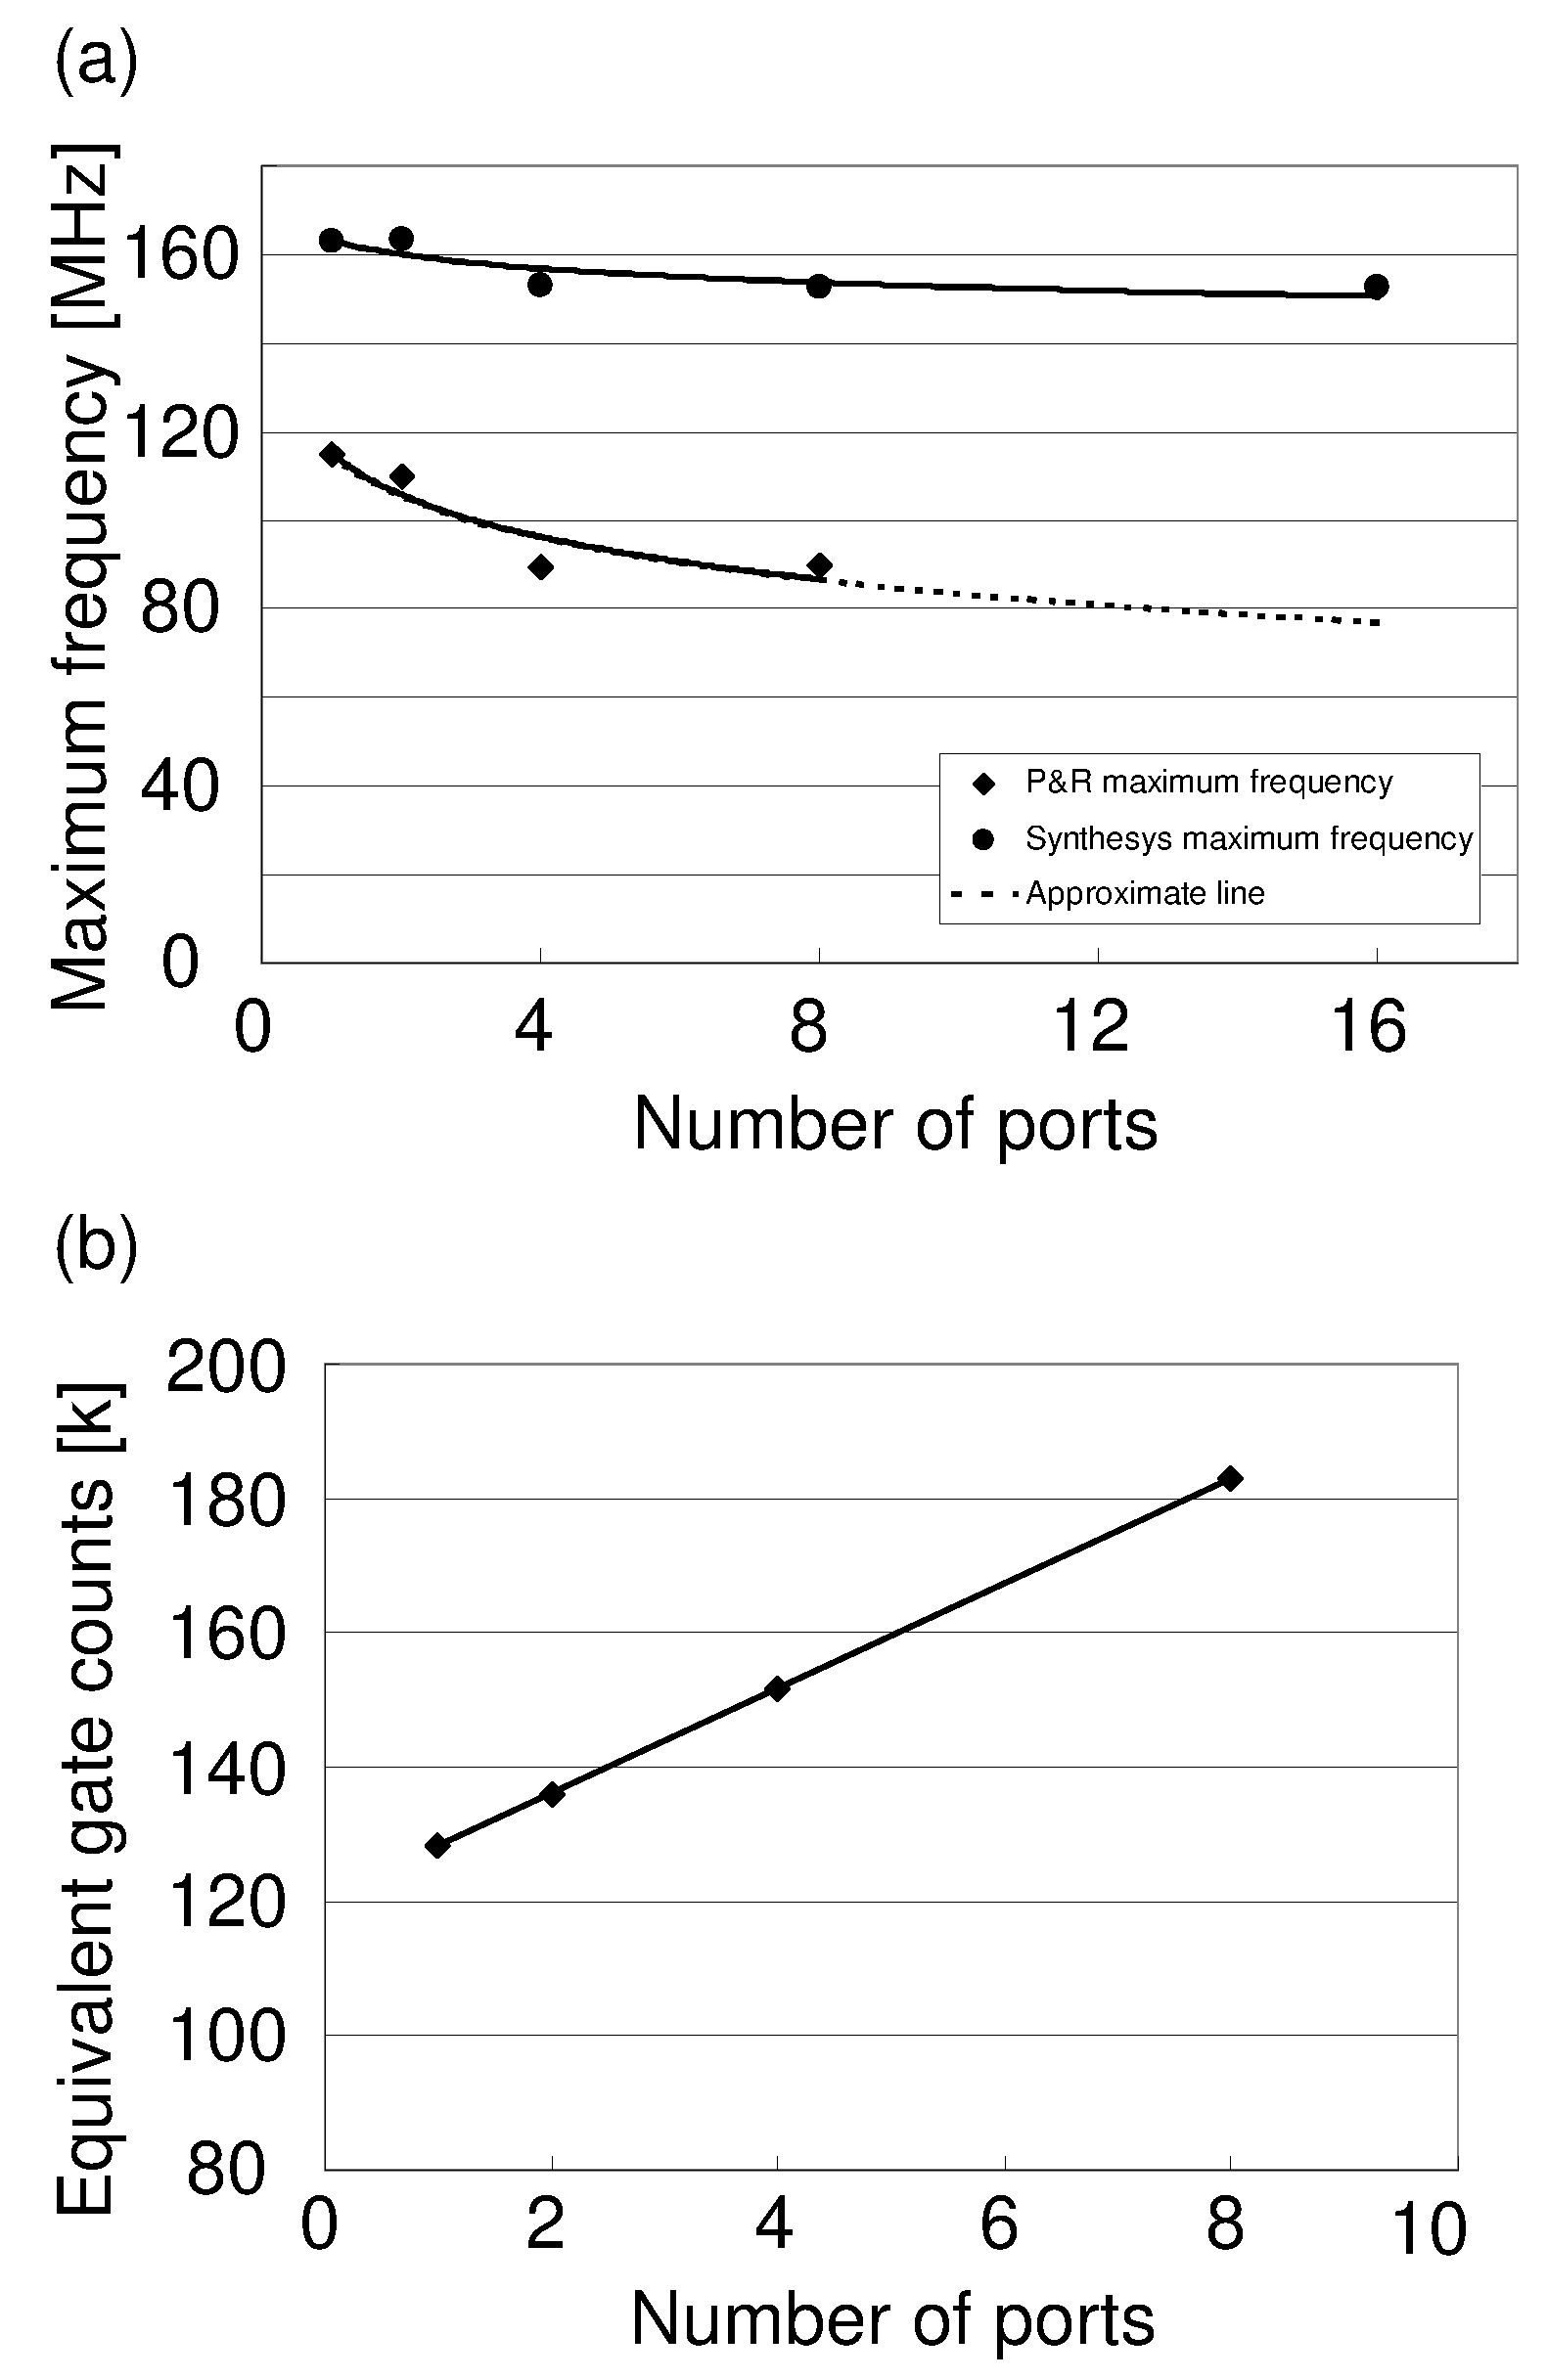
\includegraphics[width = 14cm, height = 14cm, keepaspectratio, clip]{./pics/impl_rslt_fpga.eps}
%		\caption{FMCAM implementation results for the FPGA case (Xilinx XC4VLX160) as a function of the number of ports: 
%						(a) Maximum operating frequency, (b)Total equivalent gate counts.}
		\caption{Adapted FMCAMのポート数増加に対するFPGA (Xilinx XC4VLX160)への実装結果:
						(a) 最大動作周波数, (b)ゲート数.}
		\label{impl_rslt_fpga}
		\end{center}
	\end{figure}%
%\vspace{-3mm}
% figure*

% figure*
	\begin{figure}[t]
	\centering
		\begin{center}
			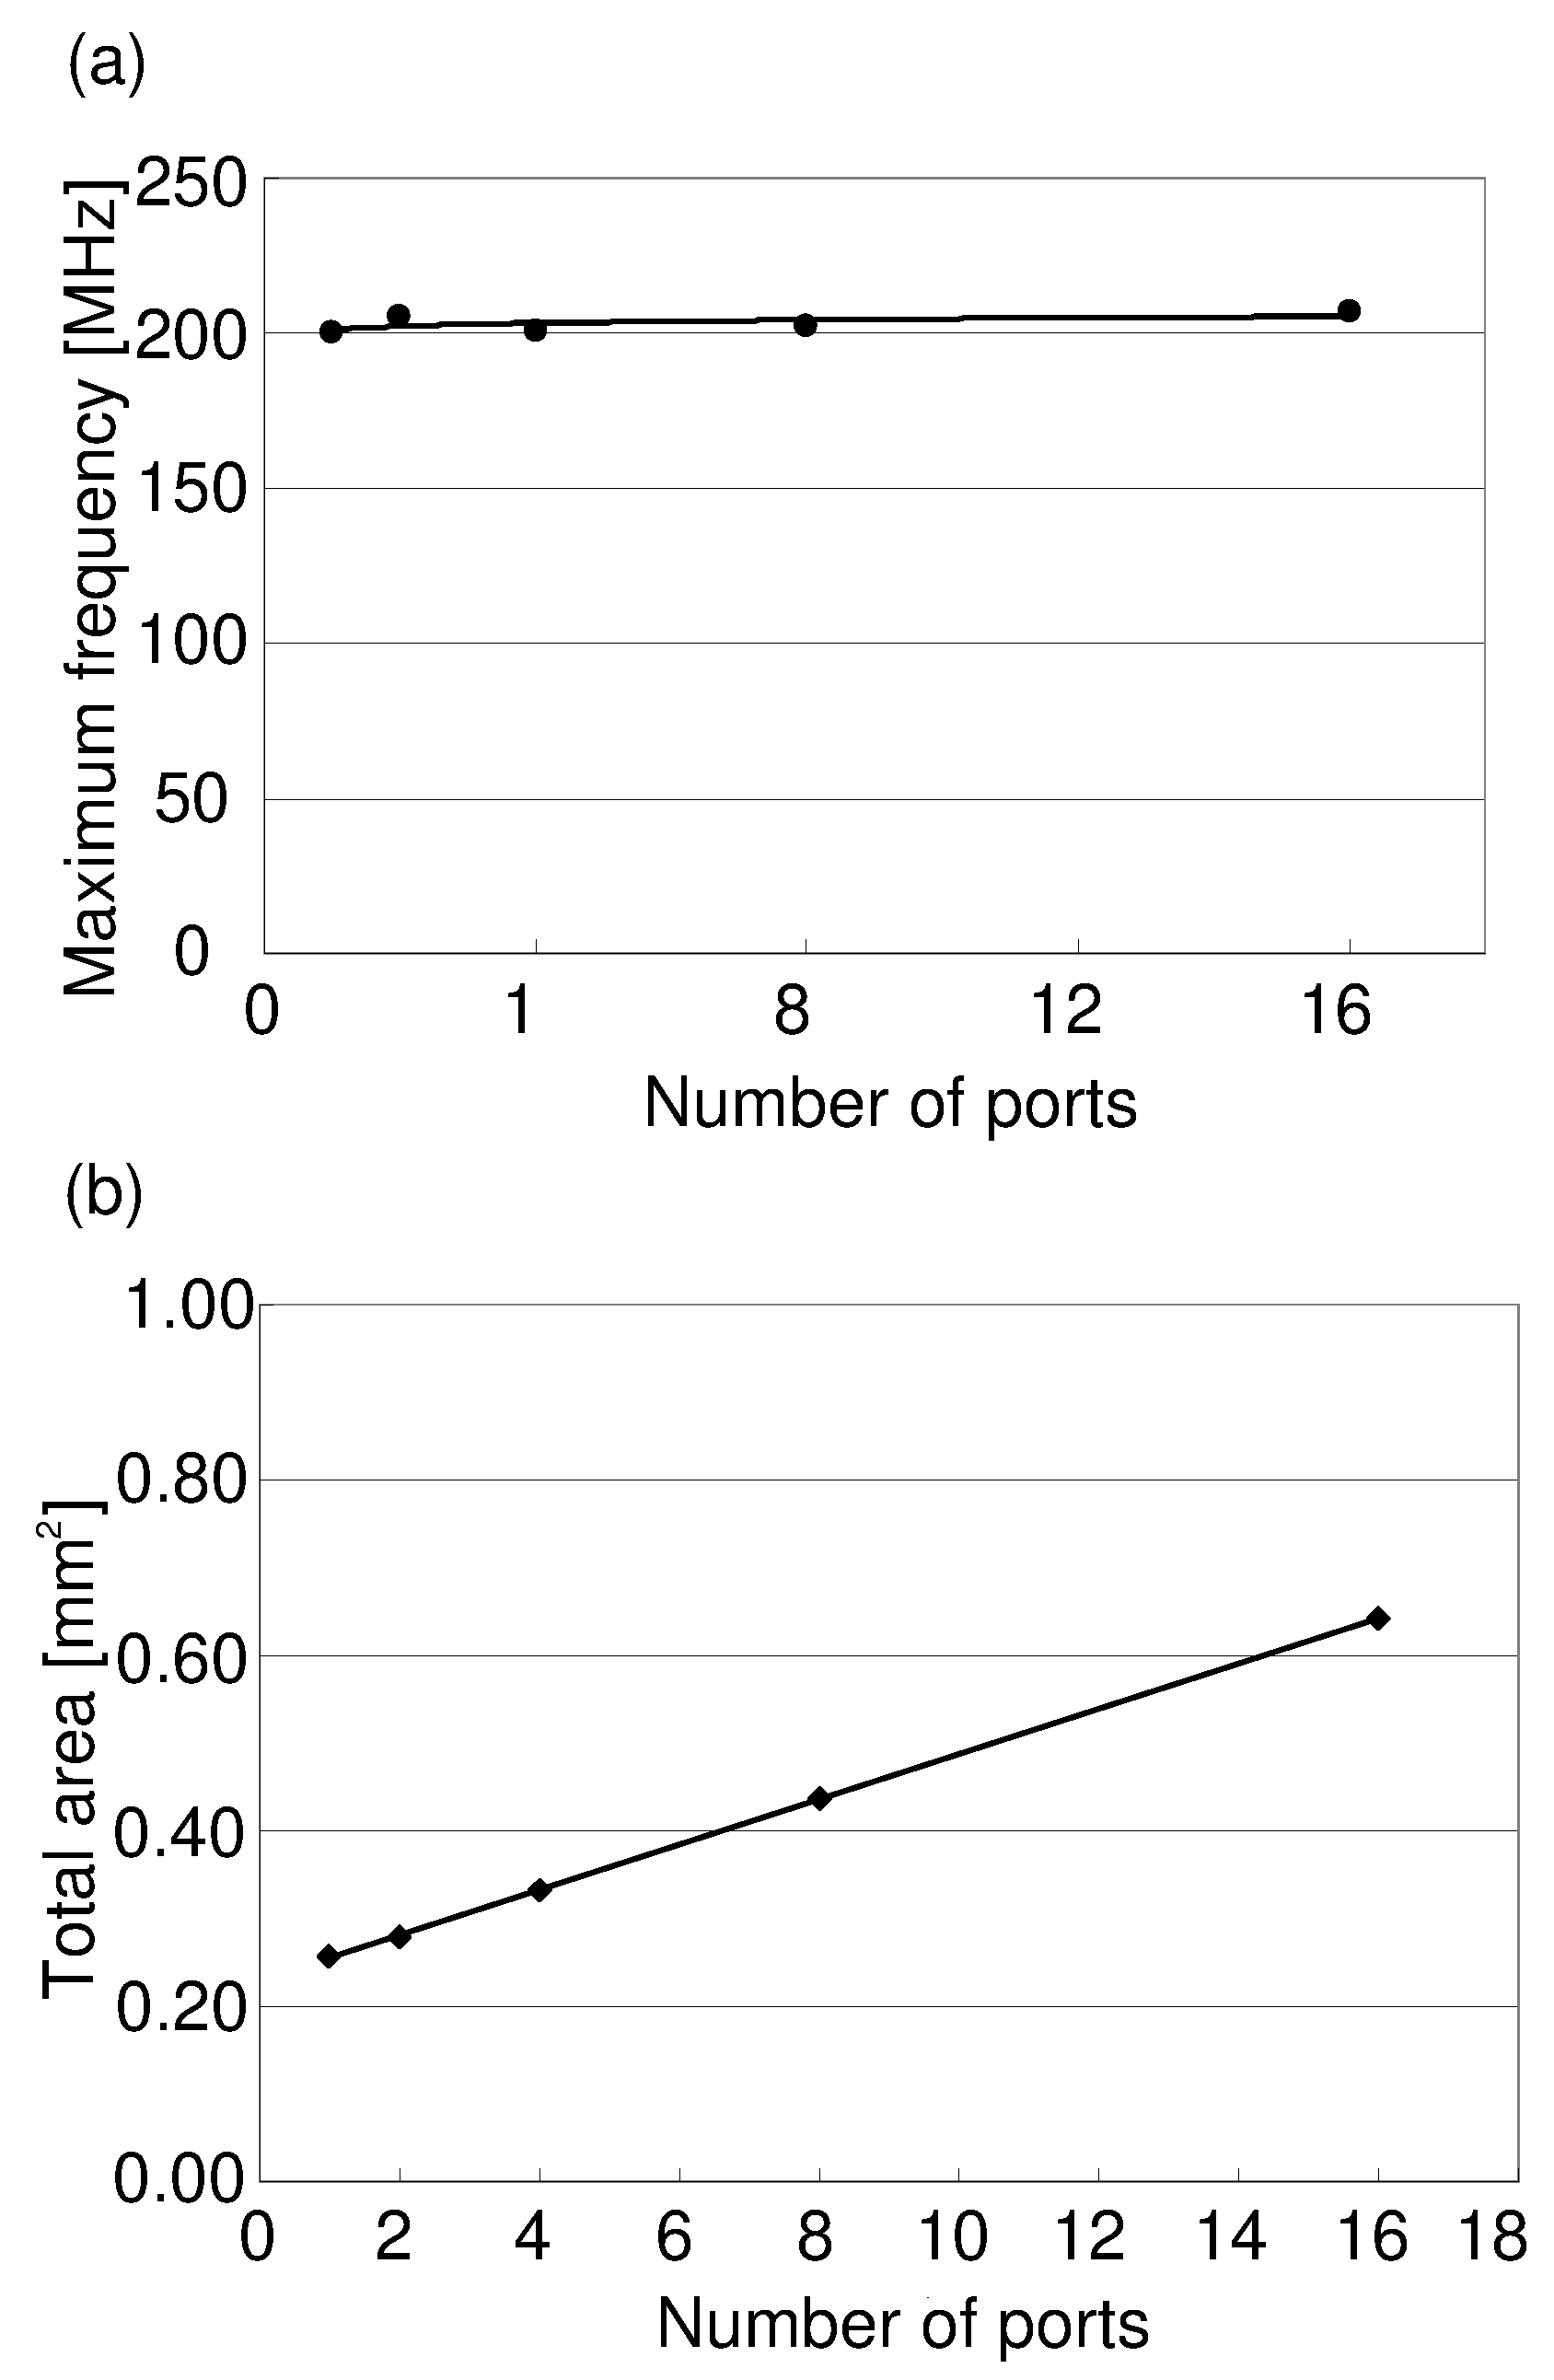
\includegraphics[width = 14cm, height = 14cm, keepaspectratio, clip]{./pics/impl_rslt_asic.eps}
%		\caption{FMCAM implementation results for the ASIC case ($90nm$ CMOS technology) as a function of the number of ports: 
%						(a) Maximum operating frequency, (b)Area consumption.}
		\caption{Adapted FMCAMのポート数増加に対するASIC (90 nm CMOS テクノロジ)への実装結果:
						(a) 最大動作周波数, (b)実装面積.}
		\label{impl_rslt_asic}
		\end{center}
	\end{figure}%
%\vspace{-3mm}
% figure*


図 \ref{impl_rslt_fpga}-(b)は,FPGAにおける配置配線後の換算ゲート数を示している.
また,図 \ref{impl_rslt_asic}-(b)は,ASICにおける論理合成後の面積を示している.
ただし,ASICにおける面積見積もりは論理合成時のものではあるが,仮想配線の面積を
加味したものとなっている.
今回の実装ではカテゴリバンク内のメモリセルをフルカスタムによるハードマクロのものではなく,
Flip-Flopベースのソフトマクロを使用した.そのため,全体の面積は大きくなっている.
一般に,マルチポートアーキテクチャ,例としてマルチポートSRAMはポートの増加に対して
実装面積が,2乗で増加することが知られている\cite{sioomp04j}.
このことがマルチポートSRAMの普及の
妨げにもなっているが,Adapted FMCAMはFPGA及びASICの実装結果共に,線形で増加することが
確認できる.その増加率は1ポートの増加に対し約9\%と低い.
これは,ポート数の増加がポートモジュールの増加,及び配線のみにとどまるからであると考えられる.

以上の結果より,Adapted FMCAMは,FPGA,ASICどちらのデバイスでも,
マルチポートの有効性を十分に発揮できる,実装にスケーラブルなアーキテクチャである見通しを得た.

\clearpage

\section{ハフマン符号化への適用と評価}
\label{lbl_cp4_adpt_fmcam_huffma}

マルチメディアデータ処理を行う従来のプロセッサにおいて,テーブルルックアップ処理の
効率的な並列化が困難であることは\ref{lbl_cp1_kousoku}節,及び\ref{lbl_cp4_intro}節で述べた.
この節では,マルチメディアデータ処理におけるAdapted FMCAMの並列テーブルルックアップ能力を
検証する.

\subsection{並列テーブルルックアップ処理の概念}
\label{lbl_cp4_adpt_fmcam_cncpt}
Adapted CAMの持つ複数の入出力ポートを利用して,並列テーブルルックアップ処理を行うためには,
マルチポートSRAMもしくは複数のSRAMと組み合わせて処理を実現する.
マルチポートSRAMには,消費電力及び面積において有効であることが報告されている
階層構造バンク型多ポートメモリ (HMA: Hierarchical Multi-port Memory)\cite{emphjm01}等
を使用することによって面積の増加を抑えることが可能である.

図 \ref{cod_proc}に,並列テーブルルックアップの概念図を示す.
ここでは,Adapted FMCAMを用いてハフマン符号化を行う例を示している.
ハフマン符号化の準備として,Adapted FMCAMには,符号化前の全データパターンを格納し,
マルチポートSRAMにはハフマン符号化テーブルを格納する.
Adapted FMCAMの各ポートには,任意のタイミングで符号化前データが入力される.
その後,符号化前データの属するカテゴリからデータパターンがロードされるため,
比較処理を行い,一致したものが見つかり次第,一致アドレスが出力される.
Adapted FMCAMの各ポートとマルチポートSRAMの各ポートは1対1で対応しているため,
マルチポートSRAMは,一致アドレスを受け取ったならば,直ちにハフマンコードを出力する.
以上の処理を行うことによって,準備する符号化前テーブルとハフマンテーブルは
1つづつであるにもかかわらず,これまで符号化が困難であったテーブルルックアップ処理を
$p$倍の並列度で実行することが可能となった.

% figure*
	\begin{figure}[tbh]
	\centering
		\begin{center}
			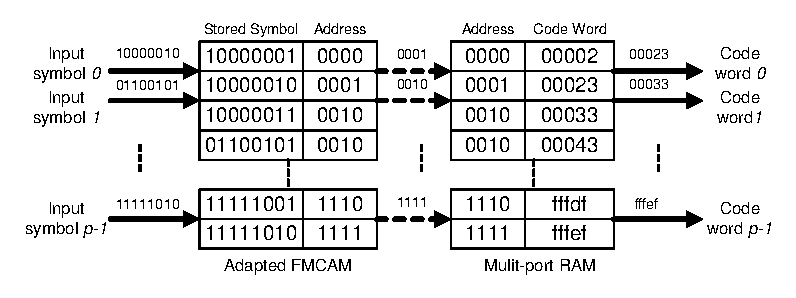
\includegraphics[width = 14cm, height = 14cm, keepaspectratio, clip]{./pics/cod_proc.eps}
%		\caption{The proposed solution of parallel table-lookup-coding.}
		\caption{並列テーブルルックアップ処理の概念図.}
		\label{cod_proc}
		\end{center}
	\end{figure}%
% figure*

\subsection{評価・検証}
\label{lbl_cp4_adpt_fmcam_rslt}

\ref{lbl_cp4_adpt_fmcam_cncpt}節で述べた,Adapted FMCAMベースの並列テーブルルックアップアーキテクチャを
ハフマン符号化に適用した結果を示す.圧縮処理に用いた画像を,図 \ref{test_pics}に示す.
これら4つの画像は,154 $\times$ 144から1,024 $\times$ 768と,大小様々なサイズを用意し,人物,動物,物体,及び風景と
一般に取り扱われることが多い被写体を選択した.
これらの画像に,Adapted FMCAMベースの並列テーブルルックアップアーキテクチャを用いて,
ハフマン符号化処理を行った.

% figure*
	\begin{figure}[tbh]
	\centering
		\begin{center}
			\includegraphics[width = 12cm, height = 12cm, keepaspectratio, clip]{./pics/test_pics.eps}
%		\caption{Test pictures.}
		\caption{ベンチマーク用画像.}
		\label{test_pics}
		\end{center}
	\end{figure}%
%\vspace{-3mm}
% figure*

得られた結果を図 \ref{clk_cycl}に示す.
各グラフの横軸はポート数,縦軸はクロックサイクル数を示している.
比較対象アーキテクチャは
Original FMCAM,及び
現在モバイル機器に搭載されている汎用品である,
2命令同時発行VLIW (Very Long Instruction Word)アーキテクチャ16 bitのDSP\cite{symdrp98, tmtmdv00, yyhskd00}である.
比較結果から分かるように,Original FMCAMは,DSPと比較してハフマン符号化処理におけるクロックサイクル数の削減を
実現している.DSPは処理の並列度を変化させることはできないため,常に一定であるのに対し,
FMCAMはポート数を増加することでその削減率は比例して向上する.
ただし,Original FMCAMはBPBP方式をそのまま適用して一致検索処理を行っているため,1回の比較に必要な処理クロックサイクル数は
16クロックと一定である.そのため画像(a)における並列度が低い1ポートに関しては,DSPによるクロックサイクル数が小さい.
これは,(a)の検証用画像がベンチマーク用として有名な被写体であり,静的ハフマン符号化テーブルによく適合しているためと考えられる.

% figure*
	\begin{figure}[tbh]
	\centering
		\begin{center}
			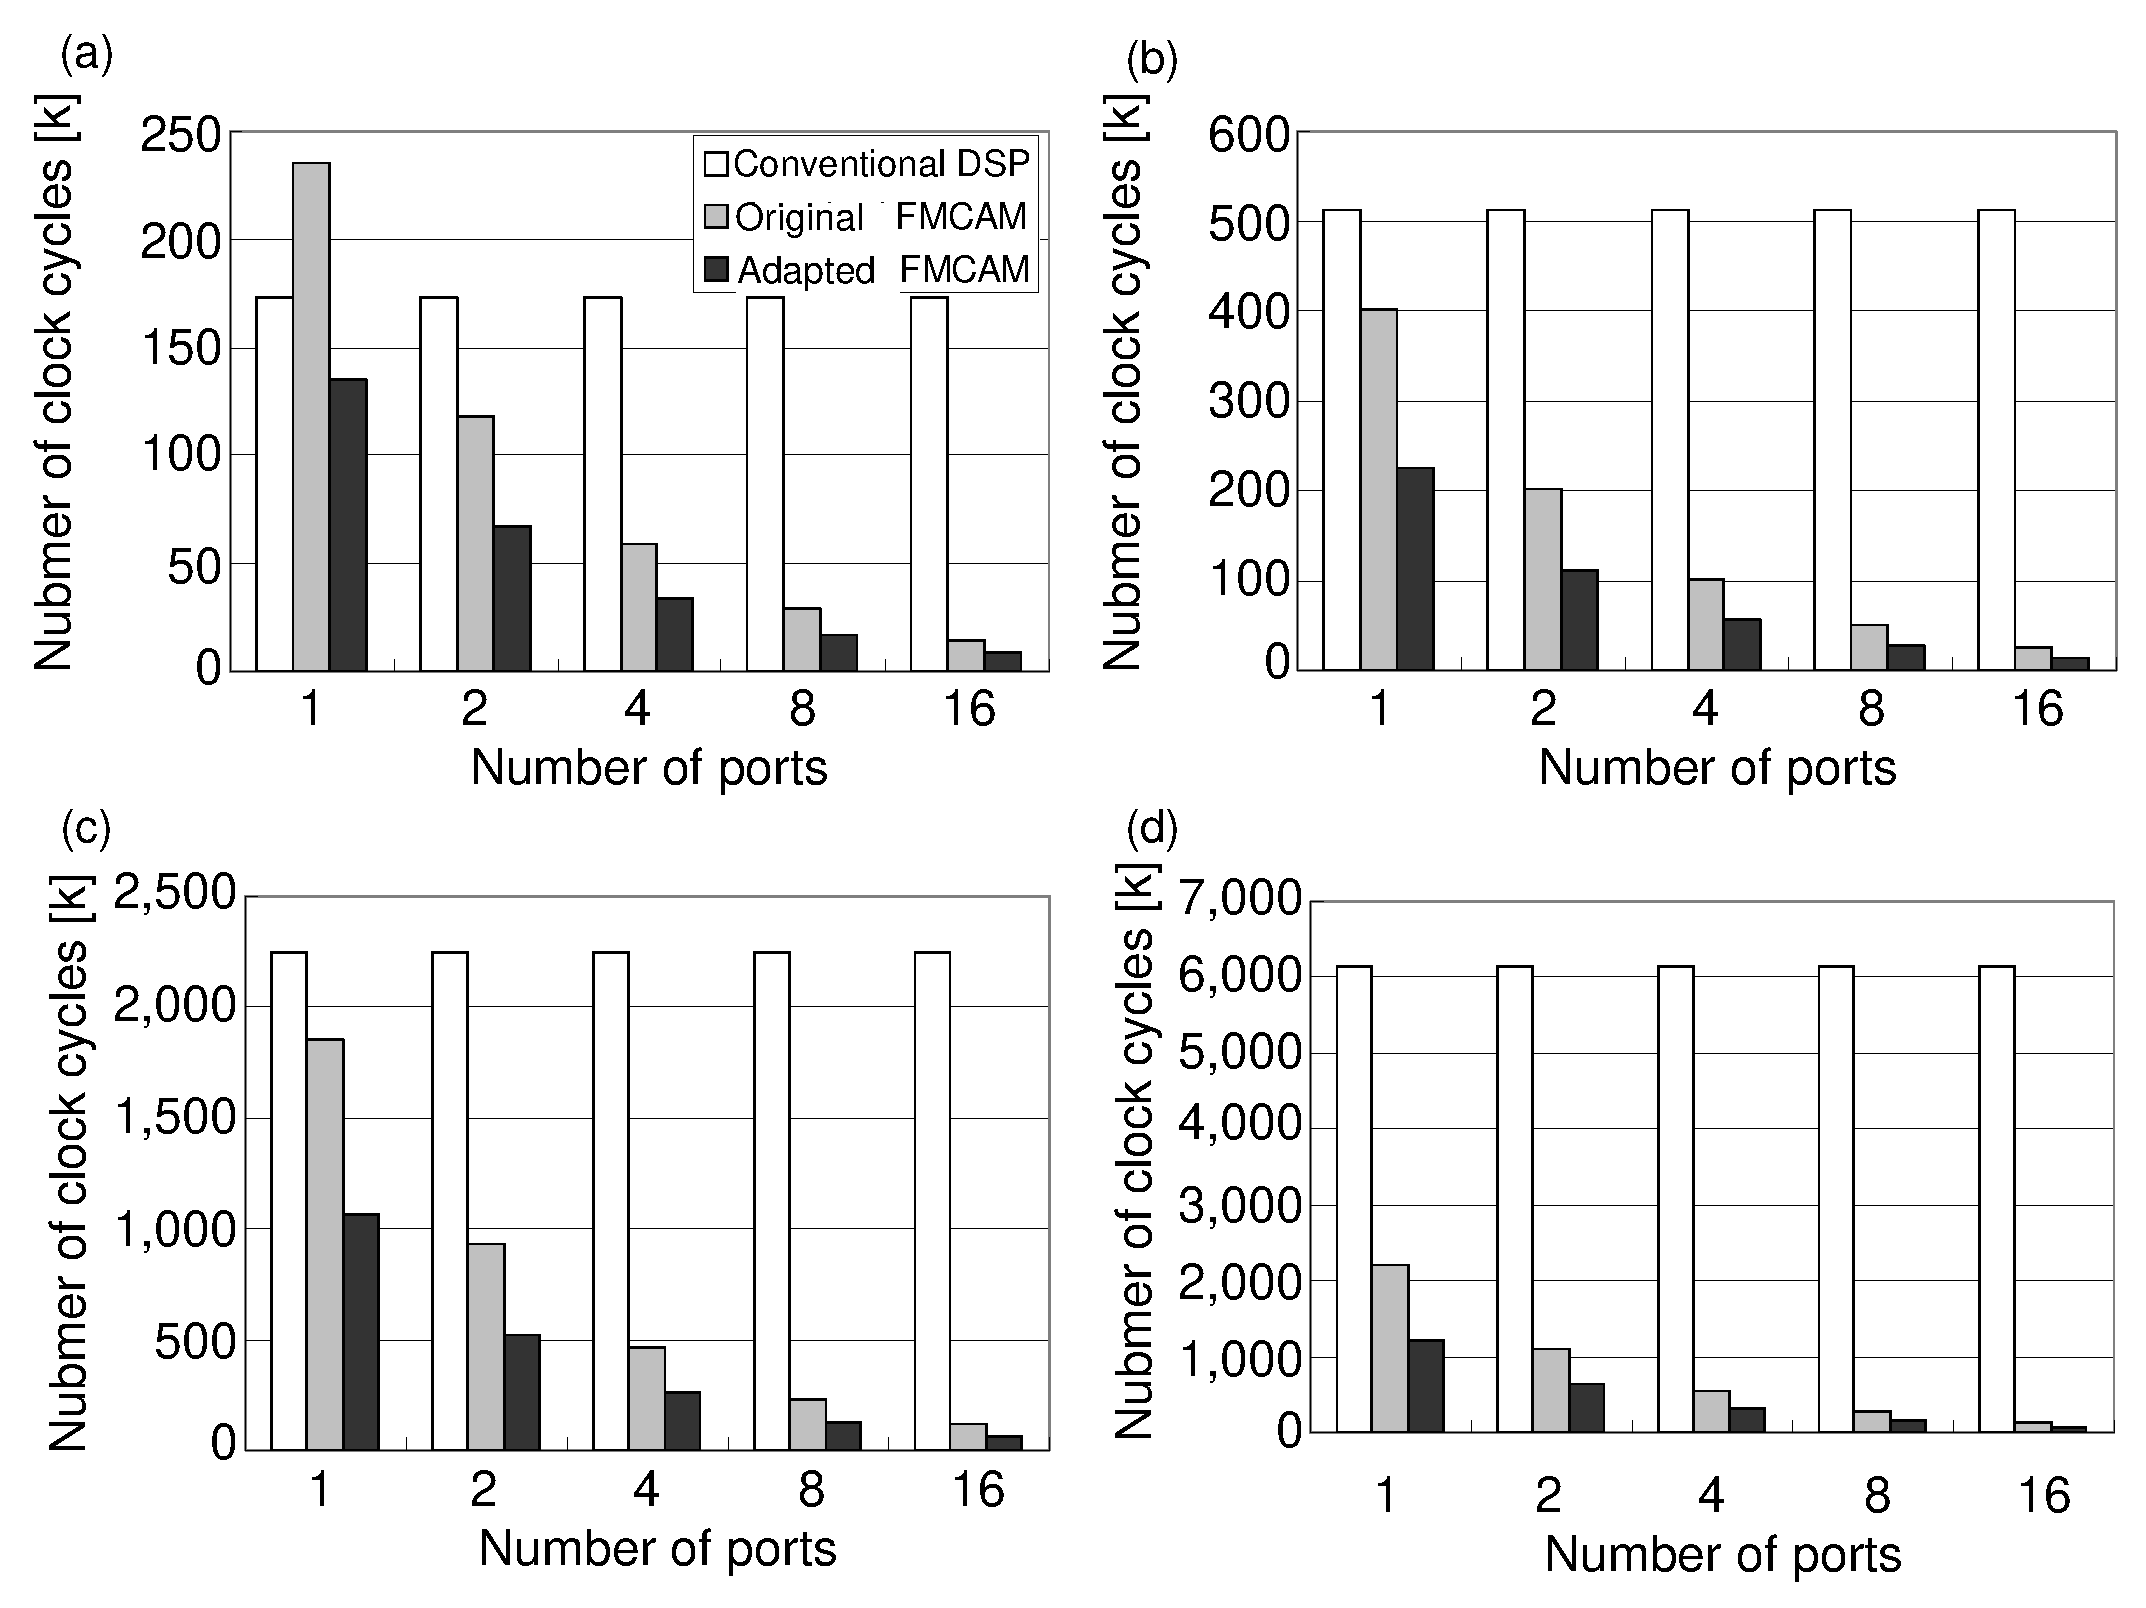
\includegraphics[width = 14cm, height =14cm, keepaspectratio, clip]{./pics/clk_cycl.eps}
%		\caption{Comparison of Huffman encoding clock cycles for FMCAM and parallel DSP solution.}
		\caption{FMCAMアーキテクチャとDSPのハフマン符号化処理クロックサイクル数の比較.}
		\label{clk_cycl}
		\end{center}
	\end{figure}%
%\vspace{-3mm}
% figure*

これらの結果に対し,Adapted FMCAMは,\ref{lbl_cp4_adpt_fmcam_mulsin}節,及び\ref{lbl_cp4_adpt_fmcam_cnt}節
で示した,シングルサーチモード,及びカウンタ値設定モードの追加によって一致検索処理にかかるクロックサイクル数の
削減を実現している.
そのため,DSP及びOriginal FMCAMと比較して大幅な比較クロックサイクル数の削減を実現した.
画像(d)のポート数16の場合にはDSPと比較して約93\%のクロックサイクル数削減を達成しており,
Adapted FMCAMの処理クロックサイクル数は各ポート数ともOriginal FMCAMに対して平均43\%の削減を実現している.
表 \ref{av_clk}に,Original FMCAMとAdapted FMCAMをポート数1から16におけるハフマン符号処理クロックサイクル数
で比較したものを示す.
どのポートにおいても,クロックサイクル数の大幅な削減を達成していることから,
Adapted FMCAMは,テーブルルックアップ処理というマルチメディアデータアルゴリズムで頻繁に行われる処理において,
BPBPアーキテクチャの本質的な問題である,一致検索時の一定クロックサイクル数
をうまく解決し,クロックサイクル数削減を達成していることが分かる.

%figure*
	\begin{table}[tbh]
	\centering
		\begin{center}
		\caption{一致検索時における,ハフマン符号化クロックサイクル数の平均値.}
%		\caption{Average of Huffman encoding clock cycles per comparison operation.}
			\includegraphics[width = 10cm, height = 10cm, keepaspectratio, clip]{./pics/av_clk.eps}
		\label{av_clk}
		\end{center}
	\end{table}%
%figure*

クロックサイクル数の削減効果を実証できたため,次に動作周波数,及び実装面積を考慮して性能比較を行う.
性能比較の指標は1秒あたりの処理回数である,MOPS (Mega Operations Per Second)を実装面積で
割った値を使用する.また,ここで扱う1回の処理とは,1つの符号化前データに対するテーブルルックアップ処理と定義する.
以下に算出式を示し,表 \ref{mops}に算出結果を示す.

%\begin{begin}
%MOPS$/$mm$^2$ $=$ $\frac{1クロックサイクルあたりの処理回数 \times 最大動作周波数[MHz]}{実装面積[mm^2]}$
%\end{end}

\begin{equation}
MOPS/mm^2 = \frac{1クロックサイクルあたりの処理回数 \times 最大動作周波数[MHz]}{実装面積[mm^2]}
\end{equation}



表 \ref{mops}は,ポート数を1から16まで変化させた場合の動作周波数,処理性能 (MOPS),実装面積,及び単位面積当たりの
性能 (MOPS$/$mm$^2$)算出結果である.
比較アーキテクチャはOriginal FMCAMと圧縮処理の評価で用いた汎用DSPである.
ただし,DSPはポートを複数持たないため,比較条件を統一する目的で
ポート数を増加した場合は並列に実装して処理することとしている.
両FMCAMとDSPの動作周波数は,約200 MHzで動作する.ここで,Original FMCAMとAdapted FMCAMの動作周波数が同一なのは,
マルチプル・シングルサーチモード,及びカウンタ値設定モードを切り替えることで,Adapted FMCAMはどちらのアーキテクチャも
実現可能であるためである.今回の評価ではAdapted FMCAMの検索モードをマルチプルサーチモードへ変更し,
カウンタ値の設定は行っていない状態でOriginal FMCAMとしている.
性能 (MOPS)は,全アーキテクチャともポート数の増加に比例して増加することが分かる.
性能 (MOPS)のみを検討すると,並列配置DSPが優れている.
しかしながら,面積の増加率がポート数の増加に比例して増加するのに対し,
両FMCAMは,\ref{lbl_cp4_adpt_fmcam_impl}節で示したように,
面積の増加が緩やかなため,単位面積当たりの性能 (MOPS$/$mm$^2$)ではAdapted FMCAMによるテーブルルックアップ符号化アーキテクチャが
効果的であることが分かる.
ポート数16の場合では,Original FMCAMと比べて1.7倍,並列配置DSPと比べて3.8倍の
向上率であった.

以上より,Adapted FMCAMはテーブルルックアップ処理を並列に行うアーキテクチャとして,
有効な構成であると考えられる.



%figure*
	\begin{table*}[tbh]
	\centering
		\begin{center}
%		\caption{Comparison of Huffman-coding processing capability 
%for FMCAM (original, adapted) and parallel DSP solutions.}
%		\caption{Comparison of Huffman-coding processing capability 
%		for FMCAM (original, adapted) and parallel DSP solutions.}
		\caption{ハフマン符号化におけるOriginal/Adapted FMCAMと並列DSPの性能比較.}
			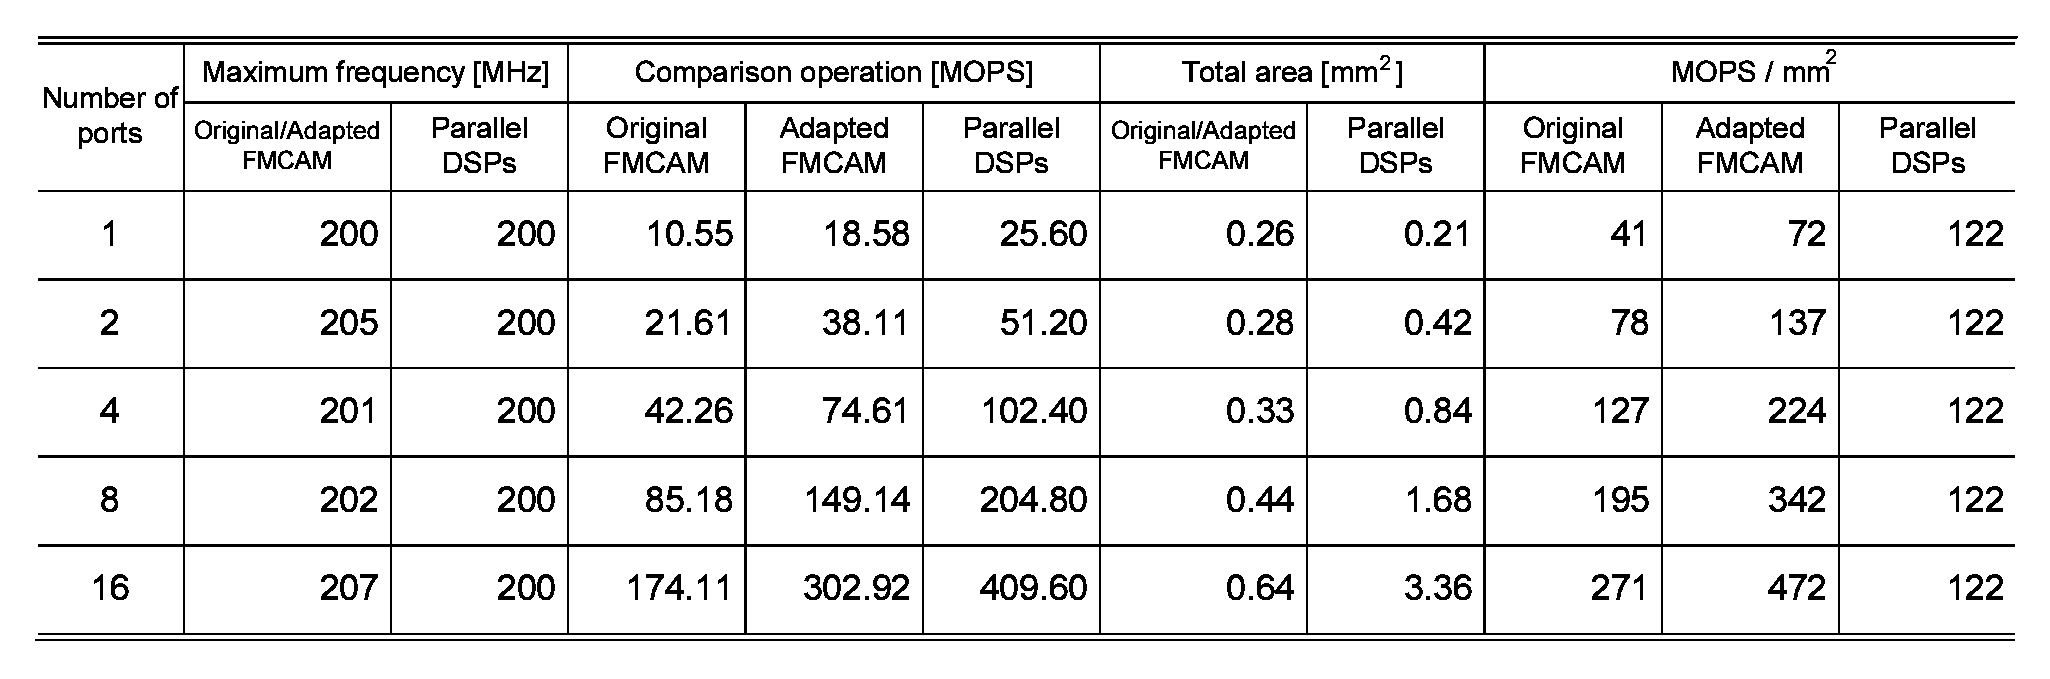
\includegraphics[width = 14.5cm, height = 14.5cm, keepaspectratio, clip]{./pics/mops.eps}
		\label{mops}
		\end{center}
	\end{table*}%
%figure*

%\clearpage

\section{リアルタイム符号化テーブル最適化アーキテクチャとの融合}
\label{lbl_cp4_adpt_fmcam_ophu}

\ref{lbl_cp4_adpt_fmcam_impl}節,及び\ref{lbl_cp4_adpt_fmcam_huffma}節等の検討で,マルチポートCAMは
テーブルルックアップ処理に対して非常に有効なアーキテクチャであることが示せた.
この節では,マルチポートCAMベーステーブルルックアップ符号化アーキテクチャの高性能化のために,
\ref{lbl_chptr3}章で示した,リアルタイム符号化テーブル最適化アーキテクチャとの融合を検討する.
これらのアーキテクチャを融合することで,マルチメディアデータを並列にリアルタイムで符号化しつつ,データサイズを
小さくできるアーキテクチャの実現が期待できる.

\subsection{処理の概要}
\label{lbl_cp4_adpt_fmcam_ophu_gaiyo}

\ref{lbl_cp4_adpt_fmcam_cncpt}節にて述べたFMCAMによる並列テーブルルックアップ処理を,
リアルタイム符号化テーブル最適化アーキテクチャに適用するには,\ref{lbl_cp3_real_opti_enc}節で示した
エンコーダ内にFMCAMとマルチポートSRAMを配置する.
図 \ref{mchrc_block}に,そのブロック図を示す.
マルチポートCAMには,FMCAMを,アクティブテーブルとシャドウテーブルには,それぞれマルチポートSRAM
を利用する.エンコーダブロックのアーキテクチャ,及び処理の概要は,ほぼ\ref{lbl_chptr3}章で述べたものと
同一であるが,オプティマイザブロックはFMCAMからの出力ポートが複数あるためデータの出現頻度を算出するために
工夫が必要となる.図 \ref{assign_mod}に並列テーブルルックアップ処理のためのアサインモジュールブロック図を示す.
FMCAMの各エントリに対応しているカウンタには,それぞれORロジックを付加し,一致アドレスを論理演算して
カウントすることとした.
このロジックを追加することによって,データの出現頻度を計算可能となる.
別々の出力ポートから同タイミングで,同一のアドレスが出力された場合は
出現頻度がまとめられることとなるが,この影響に関しては,\ref{lbl_cp4_adpt_fmcam_ophu_hyoka}にて述べることとする.
その他のシャドウテーブルアップデート及び切り替え処理アルゴリズムに関しては同一である.

% figure*
	\begin{figure}[tbh]
	\centering
		\begin{center}
			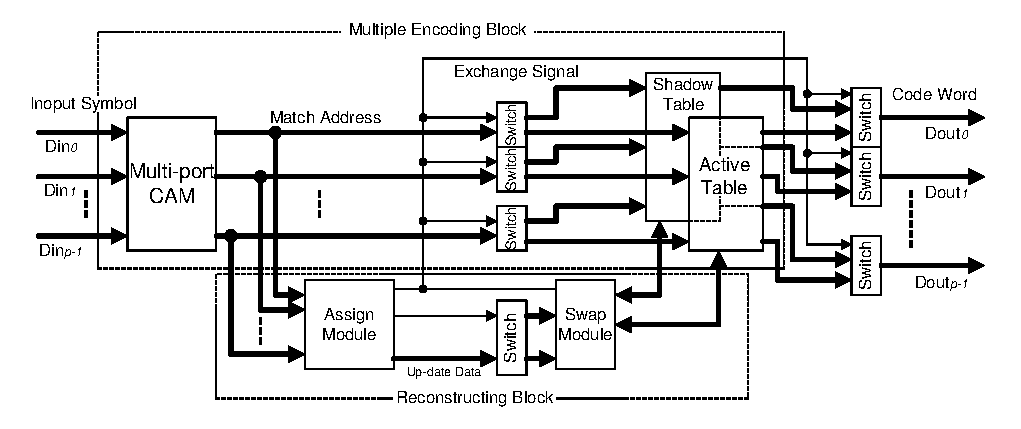
\includegraphics[width = 14cm, height = 14cm, keepaspectratio, clip]{./pics/mchrc_block.eps}
		\caption{リアルタイム符号化テーブル最適化アーキテクチャとFMCAMの融合.}
		\label{mchrc_block}
		\end{center}
	\end{figure}%
%\vspace{-3mm}
% figure*

% figure*
	\begin{figure}[tbh]
	\centering
		\begin{center}
			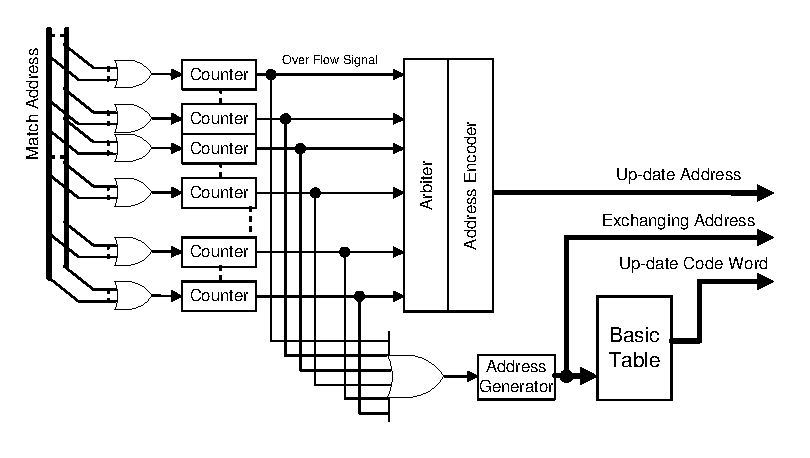
\includegraphics[width = 14cm, height = 14cm, keepaspectratio, clip]{./pics/assign_mod.eps}
		\caption{FMCAM適用時のアサインモジュールブロック図.}
		\label{assign_mod}
		\end{center}
	\end{figure}%
%\vspace{-3mm}
% figure*

\subsection{ハフマン符号化適用時における性能評価}
\label{lbl_cp4_adpt_fmcam_ophu_hyoka}

並列テーブルルックアップアーキテクチャによる,符号化テーブル最適化効果を検証するために
\ref{lbl_cp4_adpt_fmcam_huffma}節と同様に,JPEGアプリケーションにおけるハフマン符号化を対象として
性能評価を行った,なお,ハフマン符号化の圧縮率を主として検証するために,マルチポートCAMは
Original FMCAMのみを適用している.
図 \ref{mhpics}に検証に用いた画像を示す.各画像の特徴は,192 $\times$ 128から1,024 $\times$ 768までのサイズが異なる,
(A) 人物が被写体の画像,(B) 使用されている色の種類が少なく,
単純な画像,(C) 景色の画像,及び(D) コンピュータグラフィックである.
各画像とも\ref{lbl_cp4_adpt_fmcam_cncpt}節での検証と異なる条件で検証を試みた.
検証条件は色差のファクターであるC$_b$及びC$_r$のサンプリングを行わず,量子化係数は100としている.
また,Y,C$_b$及びC$_r$全てを圧縮対象のデータとしている.
%そのけっか,くろっくさいくるとがぞうのさいずもおおきくなるよね.なぜならばYCbCrの数が大きくなる.
%また,圧縮はカラーを用いているYのみではない
%これによって論文とのずれが説明できる.

% figure*
	\begin{figure}[tbh]
	\centering
		\begin{center}
			\includegraphics[width = 14cm, height = 14cm, keepaspectratio, clip]{./pics/mhpics.eps}
		\caption{ベンチマーク用画像.}
		\label{mhpics}
		\end{center}
	\end{figure}
%\vspace{-3mm}
% figure*

表 \ref{cc_dat}に検証結果を示す.比較対象アーキテクチャは,MUSIC社のシングルポートCAMであるMU9C1480A,
Xilinx社のIPコアエンコーダであるXAPP616,及びAMPHION社のSRAMベースエンコーダであるCS6100とした.
FMCAMは8ポートを実装している.
表 \ref{cc_dat}-( i )より,SRAMベースであるCS6100は,テーブルルックアップ処理を逐次的に比較して行わなければならないため,
クロックサイクル数は最も多くなっている.MU9C1480AはCAMベースであるため,比較処理を1クロックサイクルで処理でき,
XAPP616は,専用回路であるため比較にかかるクロックサイクル数は小さいものとなっている.
これらに対し,Original FMCAMは,複数のポートで処理できるためCAMや専用ハードウェアと比較しても約4分の1のクロックサイクル数で
処理であることが分かった.

%figure*
	\begin{table}[tbh]
	\centering
		\begin{center}
		\caption{処理クロックサイクル数と圧縮データサイズの算出結果.}
			\includegraphics[width = 14cm, height = 14cm, keepaspectratio, clip]{./pics/cc_dat.eps}
		\label{cc_dat}
		\end{center}
	\end{table}%
%\vspace{-5mm}
%figure*


次に,表 \ref{cc_dat}-( ii )より,データの圧縮サイズの検証を行った.Original FMCAM以外のアーキテクチャは,静的ハフマン符号化を
実装しているため同一の値となる.
今回の検証で用いた画像は,単純な画像,もしくはサンプル画像が多いため静的ハフマン符号化に用いている
既存のテーブルに適している画像が多い.
それにもかかわらず,どの画像もリアルタイム符号化テーブル最適化アルゴリズムの効果が現れており,
画像サイズの圧縮効果が確認できている.特に画像(D)に関しては,約20\%の削減を達成している.
これより,別々の出力ポートから同タイミングで,同一のアドレスが出力された場合の影響は少ないもの
と考えられる.

以上の検証よりマルチポートCAMベースのテーブルルックアップ符号化アーキテクチャと,
リアルタイム符号化テーブル最適化アーキテクチャとの融合は,テーブルルックアップ処理を
高速,高圧縮で処理できることが確認できた.
これにより,マルチメディアデータ処理においてボトルネックとなっていたテーブルルックアップ処理を
高速かつ高圧縮に処理できることが期待できる.




